\clearpage

\def\chaptertitle{Performance Evaluation}

\lhead{\emph{\chaptertitle}}

\chapter{\chaptertitle}
\label{ch:performance-evaluation}

In this chapter, we begin by discussing the underlying server hardware configuration, and the assumptions made before beginning the auto-scaling experiments in section \ref{sec:ch6-hardware-assumptions}. The cluster configuration, which involves the resource divisions between servers, overall cluster architecture, and deployment resources is discussed in section \ref{sec:ch6-cluster-config}. The experimental setup which details the SLA categories, its latency values, and an overview of the two experiments to be conducted are discussed in section \ref{sec:ch6-exp-setup}. Following this, the workload which was generated to test the two experimental conditions along with a brief analysis of the latency graph is provided in section \ref{sec:ch6-exp-workload}. After this, an overview of the three baseline algorithms which were used to compare the performance of the proposed hybrid autoscaler is outlined in section \ref{sec:ch6-baseline-algos}. Finally, the experimental results are shown in sections \ref{sec:ch6-request-latency-eval}, \ref{sec:ch6-cpu-workload-eval}, and \ref{sec:ch6-sla-violation-eval} respectively.

\section{Assumptions and Virtual Machines Setup}
\label{sec:ch6-hardware-assumptions}

For the underlying virtual machine (VM) setup, servers in the Melbourne Research Cloud \footnote{\url{https://docs.cloud.unimelb.edu.au/}} were leveraged to deploy micro-services on. The setup consisted of 6 VMs, using a total of 24 CPU cores and 80GB of memory. These servers were separated into a cloud and an edge layer. The servers on the cloud layer have a substantially higher amount of CPU cores and memory assigned compared to the servers in the edge layer, to simulate the scarcity of resources in the edge layer. The cloud layer also contained a 200GB persistent storage volume, while the edge layer did not. This allowed the cloud layer to hold all the Prometheus data, while the edge layer had to store the time series in the RAM to depict the scarcity of resources further. Finally, a simulated latency was added between inter-layer server communication to mimic the perceived distance between edge nodes and large data centres.\par

Each server consists of an Ubuntu 22.04 \footnote{\url{https://releases.ubuntu.com/jammy/}} operating system. Kubernetes v1.28.2 \footnote{\url{https://kubernetes.io/releases/}} is used as the container orchestration technology behind the experimental micro service setup. CRI-O was installed on the Kubernetes nodes as the container runtime of choice for running resource nodes. Finally, for inter-pod communication on the cluster to occur, an open-source project known as Flannel \footnote{\url{https://github.com/flannel-io/flannel}} was deployed.\par

For maximum flexibility in modifying and monitoring the underlying architecture, a bare-metal implementation of Kubernetes was used, instead of ready-made solutions available from Amazon or Google. The control plane was deployed on the cloud layer, while the data plane was on the edge layer. Furthermore, several assumptions were made before proceeding with the experimentation:

\begin{itemize}
    \item The only auto-scaling performed would be horizontal pod auto-scaling. Vertical and cluster auto-scaling were out of the scope of this project.
    \item The pods on which auto-scaling is not applied would have the maximum possible resource allocation, so as to remove the chances of bottleneck.
    \item At no point in the experiment would a node be taken down, or new node be added.
    \item The autoscaler assumes that every node in the edge layer is an equally likely candidate for scheduling pods on.
\end{itemize}

\section{Cluster Configurations}
\label{sec:ch6-cluster-config}

The VMs were divided into the cloud and edge layer as depicted in table \ref{tab:cluster-hw-overview}. The control plane was further divided into two servers, one for handling the Kubernetes control plane scheduling, API service, and etcd deployments, and the other for storing the Prometheus database, along with the micro-service Jaeger metrics collection. The edge layer consisted of four servers with far substantially fewer resources, to depict the difference in computing power. The network layer between the edge and cloud deployments also contained a simulated latency to denote the perceived geographical distance between them.\par

%TC:ignore
\begin{table}
    \caption{Cluster architectural layout}\label{tab:cluster-hw-overview}
    \centering
    \begin{tabular}{|l|l|l|l|}
        \hline
        Node & Layer & CPU (cores) & Memory (GB)\\
        \hline
        Control-Plane-K8s & Cloud & 8 & 32\\
        Control-Plane-DB  & Cloud & 8 & 32\\
        Data-Plane-1      & Edge  & 2 & 4\\
        Data-Plane-2      & Edge  & 2 & 4\\
        Data-Plane-3      & Edge  & 2 & 4\\
        Data-Plane-4      & Edge  & 2 & 4\\
        \hline
    \end{tabular}
\end{table}
%TC:endignore

The cloud and edge nodes were differentiated through Kubernetes through the internal labeling system. A key \textit{type} with the value either \textit{cloud} or \textit{edge} was added to each node. This would enable the scheduler to consider restricting the deployment of pods to particular nodes automatically. For example, the Prometheus deployment would only be deployed on the node of the type cloud. This process is known as \textit{node affinity} \cite{santos2019towards}.\par

There were several options to deploy the social media application to Kubernetes. Manually cloning them from the repository, creating the custom resource definitions (CRDs), and deploying the YAML files was an option that gave maximum flexibility, but was difficult to debug if things went wrong. Due to this, the Kubernetes package manager Helm was used. Helm \footnote{\url{https://helm.sh/}} is another open-source project whose primary goal involves streamlining the installation, maintenance, and removal of Kubernetes deployments. This is achieved through the use of a Helm chart, which details the configuration of the project, and how to update and access it.\par

Therefore, the social media application was the first to be deployed on Kubernetes. However, before deploying the application, the primary deployments to be tested need to be configured. Based on the \textit{wrk2} benchmark that was discussed above, two APIs were identified. One was a GET call to the user's home timeline, and the other was a POST method made by the user to create a post.\par

First, the social network with default configuration values was installed using the helm command below:

\begin{lstlisting}[
  caption={Social network installation using Helm},
  captionpos=t,
  label={lst:social-network-helm-install},
  language=bash
]
$ helm install social-media \
/DeathStarBench/socialNetwork/helm-chart/Chart.yaml -n default
\end{lstlisting}

With the social media network now deployed, a workload for both GET and POST commands was invoked to generate the latency trace on Jaeger, as depicted in listing \ref{lst:wrk2-api-calls}.

\begin{lstlisting}[
  caption={Generate Jaeger trace},
  captionpos=t,
  label={lst:wrk2-api-calls},
  float=ht,
  language=bash
]
$ WRK2="/DeathStarBench/wrk2/wrk -D exp -t 1 -c 1 -d 1 -L -s -R 1"
$ HT=./wrk2/scripts/social-network/read-home-timeline.lua
$ CS=./wrk2/scripts/social-network/compose-post.lua
$ IP=$(kubectl get svc nginx-thrift --template '{{.spec.clusterIP}}')
$ PORT=8080
$ $WRK2 $HT http://$IP:$PORT/wrk2-api/home-timeline/read
$ $WRK2 $HT http://$IP:$PORT/wrk2-api/post/compose
\end{lstlisting}

With the traces generated, the deployments that require auto-scaling could be identified for each. From the Jaeger traces generated in figure \ref{fig:ht-cp-trace}, it was clear that the two deployments highlighted in pink, namely \textit{home-timeline-service}, and \textit{compose-post-service}, were the major bottlenecks in GET and POST API processing respectively, having to serve multiple child deployments simultaneously. This made them the most important deployments for auto-scaling. Therefore, the helm deployment was updated to assign auto-scaling resource limits to them. The resources were assigned in a realistic manner consistent with edge deployments and based on the number of components each deployment answered to. Listing \ref{lst:deploy-resource-update} shows the CPU resources assigned to both deployments.\par

\begin{figure}[htb]
    \centering
    \caption{API trace for \textit{home-timeline-service} and \textit{compose-post-service}}
    \label{fig:ht-cp-trace}
    \begin{minipage}{0.25\linewidth}
        %\caption{Home Timeline API trace}
        %\label{fig:home-timeline-trace}
        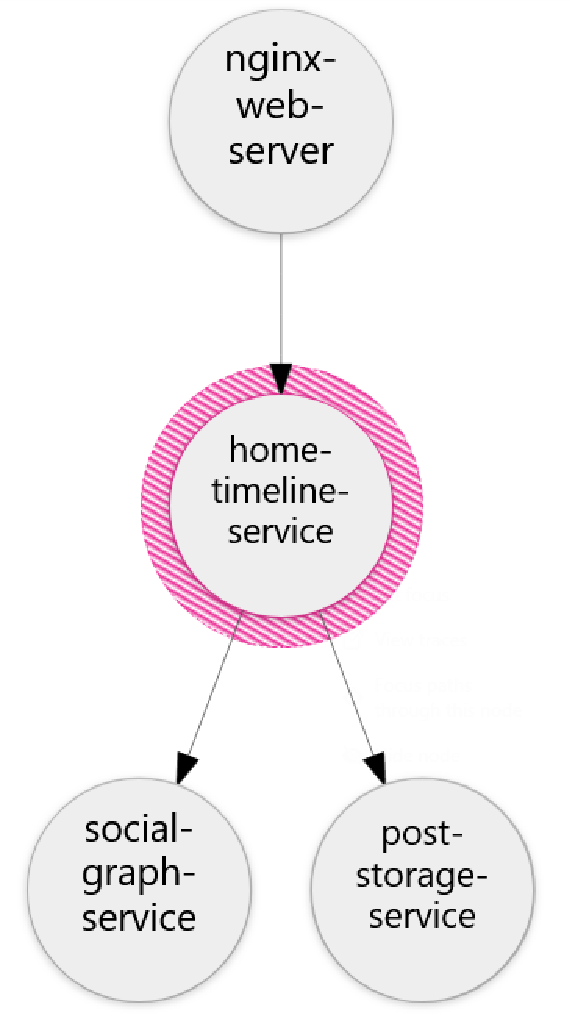
\includegraphics[width=1.0\linewidth]{Figures/Home-Timeline-GET-Trace.pdf}
    \end{minipage}\hfill
    \begin{minipage}{0.75\linewidth}
        %\caption{Compose Post API trace}
        %\label{fig:compose-post-trace}
        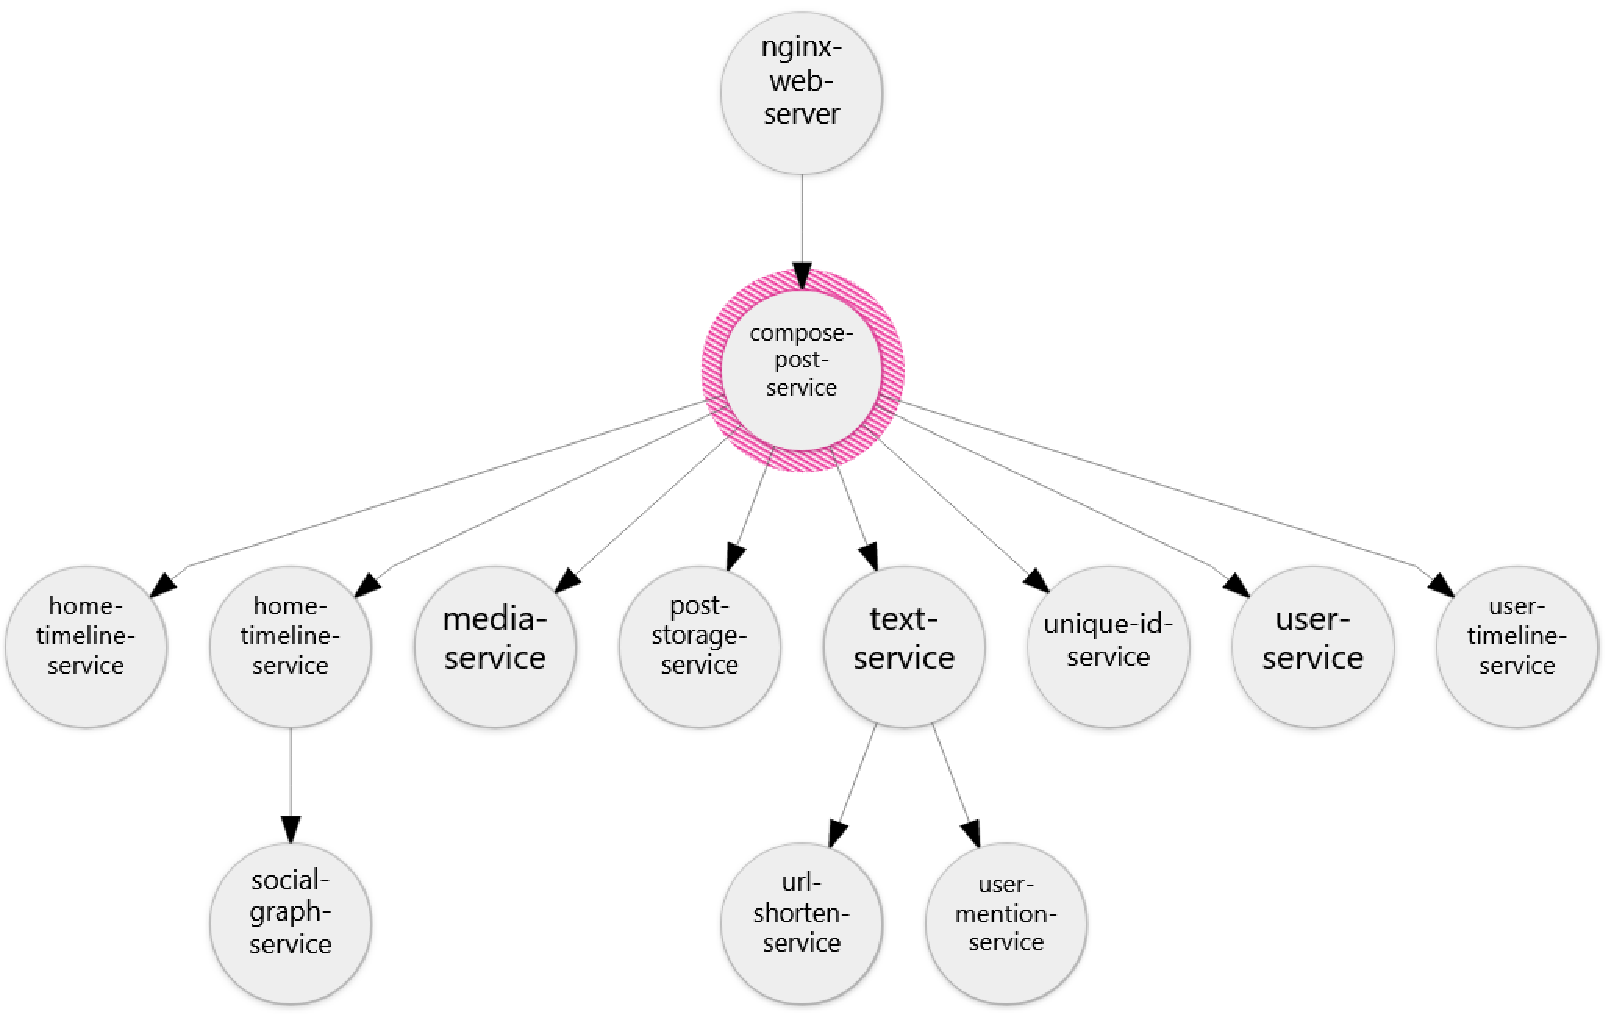
\includegraphics[width=1.0\linewidth]{Figures/Compose-Post-POST-Trace.pdf}
    \end{minipage}
\end{figure}

\begin{lstlisting}[
  caption={Update resources for bottlenecked deployments},
  captionpos=t,
  label={lst:deploy-resource-update},
  language=bash
]
$ helm upgrade social-media \
/DeathStarBench/socialNetwork/helm-chart/Chart.yaml -n default \
--set-string home-timeline-service.container.resources="requests: 
      cpu: "15m"
    limits:
      cpu: "15m"" \
--set-string compose-post-service.container.resources="requests: 
      cpu: "30m"
    limits:
      cpu: "30m""
\end{lstlisting}

\section{Experiment Setup}
\label{sec:ch6-exp-setup}

Two independent experiments were conducted to validate the performance of the hybrid autoscaler. The social media application was first tested using the GET API to autoscale the \textit{home-timeline-service} deployment. Then, a more demanding as well as challenging workload was applied to the POST API for auto-scaling the \textit{compose-post-service} deployment. For both these experiments, the workload generation algorithm was used to create realistic daily workloads and tested over a period of five days.

According to Nilsson and Yngwe \cite{nilsson2022api}, their research concluded that user experience was negatively affected by higher API latency. This leads to a cascading issue of lower revenue growth and profit. Their research found three latency brackets where the user experience changes.

\begin{itemize}
    \item A response time of at least \textit{100 milliseconds} was considered by the user to be instantaneous. This is the best case scenario.
    \item A response time of up to \textit{1 second} was noticed by the user as a slight delay, however their user experience was not significantly interrupted.
    \item A response time exceeding \textit{10 seconds} was deemed to cause the user to lose focus, and thus disrupted their user experience.
\end{itemize}

Based on this research, it was determined that the flexible, moderate, and strict SLA constraints discussed in section \ref{sec:ch4-problem-overview} would be bound within the values $SLA(c) \in [100ms, 1000ms]$.\par

The flexible SLA constraint was the primary focus of the experiment. This threshold was chosen as it is the most common threshold used for IoT applications, and thus provide a good benchmark for application performance. However, a moderate and strict SLA constraint would also be chosen and tested to compute the SLA violation rates for the algorithm. The SLA values are shown in table \ref{tab:experiment-sla-values}.\par

%TC:ignore
\begin{table}
    \caption{Experimental SLA constraints}\label{tab:experiment-sla-values}
    \centering
    \begin{tabular}{|l|l|l|}
        \hline
        SLA Type & GET latency constraint (ms) & POST latency constraint (ms)\\
        \hline
        Flexible    & 150   & 1000\\
        Moderate    & 125   & 900\\
        Strict      & 100   & 800\\
        \hline
    \end{tabular}
\end{table}
%TC:endignore

For the proposed hybrid algorithm to achieve these auto-scaling goals within the SLA constraints, the auto-scaling subsystems were configured as follows. The reactive autoscaler would check if the CPU utilization of the deployment was exceeding the auto-scaling threshold. This threshold would vary for each of the experiments as required. If this threshold was breached, it would scale up based on the cooldowns and tolerations set. The proactive autoscaler on the other hand would check if the forecasted CPU utilization in the next 20 minutes was going to breach the auto-scaling threshold, and if so, would autoscale with the same configured parameters as the reactive one. The controller would store the total CPU utilization of the deployment as a time-series for a maximum of seven days, and constantly check for SLA violations to tweak the hyper-parameters of the forecaster as discussed above in section \ref{subsec:ch5-auto-daemon-subsection}.\par

\section{Baseline Algorithms}
\label{sec:ch6-baseline-algos}

To measure the effectiveness of the hybrid autoscaler, three baseline algorithms were chosen for comparison. All three would autoscale at the same CPU auto-scaling threshold to maintain consistency. Furthermore, these algorithms would be implementations based on the ones discussed in chapter \ref{ch:lit-review}.\par

\begin{itemize}
    \item The first is the \textbf{Default Kubernetes Horizontal Pod Autoscaler}. No modifications to the configuration are made, thus the scale-up cooldown is 0 seconds, while the scale-down is 300 seconds. Additionally, the autoscaler has no knowledge of the workload distribution or SLA violations on the edge nodes.
    \item The second baseline is an implementation of the reactive \textbf{Traffic Aware Horizontal Pod Autoscaler} (THPA) created by Phan \textit{et al}. \cite{phan2022traffic}. This autoscaler scheduler will compute the ratio of workloads being exerted on the different edge nodes with the deployment pods. Once it does so, it will scale these resources in a commensurate proportion.
    \item Finally, the third baseline implementation is the \textbf{Proactive Pod Autoscaler} (PPA) devised by Ju \textit{et al}. \cite{ju2021proactive}. This algorithm was an open-ended implementation that enabled the user to plugin a deep learning model of their choice. The PPA architecture consists of three sub-sections, the formulator, evaluator, and updater. An LSTM model is injected into the autoscaler as the model file. This LSTM implementation is similar to the one used in the hybrid autoscaler, however, it differs in two key elements. First, the LSTM does not expect pre-processed data without noise and thus deals with more complex time-series data. Secondly, due to this additional computation, the LSTM contains a deeper architecture layer with more neural network units. This is required as the algorithm has to correctly predict the complete future workload since there is no reactive autoscaler to fall back on. Over a fixed interval, the algorithm continuously loops through the time-series data and saves the forecast result to a metrics file. The evaluator takes these outputs from the metrics file, along with the LSTM from the model file to predict the number of pods to assign in advance, and requests the Kubernetes scheduler for scaling through the API Service. A second loop, known as the update loop, then updates the LSTM model using the latest forecast, and clears the metrics file. The hyper-parameters are carefully tuned to ensure that the model does not underperform. Finally, the PPA architecture does not take into account SLA compliance, and thus SLA metrics are not provided as feedback for hyper-parameter tuning.
\end{itemize}

\section{Experimental Workload}
\label{sec:ch6-exp-workload}

In the first experiment, the IoT workload generation algorithm was configured to create a workload aimed at mimicking GET requests. By doing so, the \textit{home-timeline-service} deployment became the bottleneck receiving all of the requests and thus could be tested using the proposed hybrid autoscaler, as well as the three baseline algorithms. As explained above, the auto-scaling threshold for all four algorithms was set to 50\% total CPU utilization on the deployment, and the SLA latency threshold was set to the flexible threshold of 150 milliseconds.\par

\begin{comment}
\begin{figure}[htb]
    \centering
    \caption{Total CPU utilization for home-timeline-service}
    \label{fig:exp1-workload}
    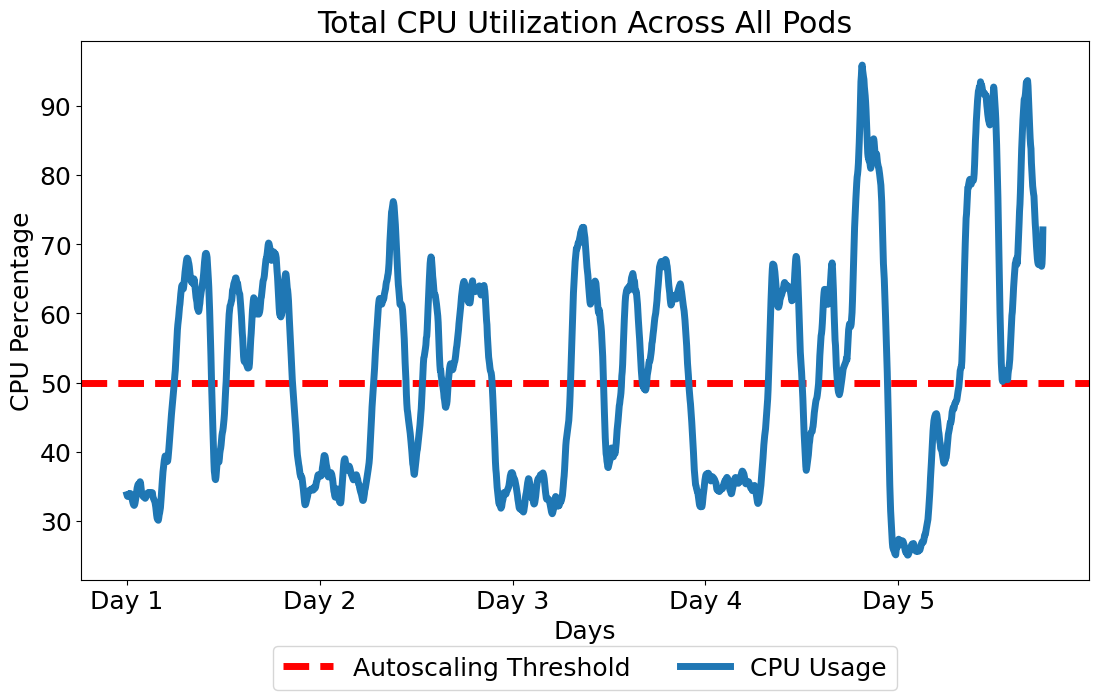
\includegraphics[width=0.6\linewidth]{Figures/GET-Total-CPU.pdf}
\end{figure}
\end{comment}

\begin{center}
\begin{minipage}{\linewidth}
    \captionof{figure}{Total CPU utilization for \textit{home-timeline-service}}
    \label{fig:exp1-workload}
    \begin{tikzpicture}
        \begin{axis}[
            height=0.4\linewidth,
            width=\linewidth,
            xmin=0,
            xmax=2460,  % Make xmax 150 above the final xtick
            ymin=0,
            ymajorgrids=true,
            yminorgrids=true,
            xmajorgrids=true,
            xminorgrids=true,
            grid style=dashed,
            xlabel={Time (Days)},
            ylabel={CPU Usage (\%)},
            legend style={at={(0.5,-0.3)},anchor=north,legend columns=-1},
            xticklabels={Day 1, Day 2, Day 3, Day 4, Day 5},
            xtick={570, 1030, 1510, 1950, 2370}
        ]
            \addplot+[RoyalBlue, mark=none] table [x=xtick, y=value, col sep=comma] {Data/GET-Total-CPU.csv};
            \draw[red, thick, dashed] (axis cs:0, 50) -- (axis cs:2460, 50);
            \legend{CPU Usage}
            \addlegendimage{line width=0.3mm, dashed, color=red}
            \addlegendentry{Autoscaling Threshold}
        \end{axis}
    \end{tikzpicture}
\end{minipage}
\end{center}

Figure \ref{fig:exp1-workload} shows the total CPU workload that was generated by algorithm \ref{alg:work-gen} on the \textit{home-timeline-service} deployment. The data was generated for a total of five days. Throughout the five days, approximately \num[group-separator={,}]{2550000} requests in total were sent to the edge deployment. The daily peak remained at approximately the same percentage but then increased significantly in the last two days. This could be interpreted as a depiction of how social network requests may look on the weekends. The total CPU utilization never exceeded 95\% of the total allocated resources shown in listing \ref{lst:deploy-resource-update}. This is expected of a GET request, as while the deployment has to open a connection to the sub-deployments to receive the response, a GET request is typically a database SELECT statement, which takes a comparatively less amount of time as opposed to other operations. This means that the deployment can quickly receive the response from its child components, send the response up to the requester, and then close the connection. Once the connection is closed, all the resources associated with it are freed. Because this operation is so quick, multiple concurrent connections are typically not open, and thus the CPU utilization is not significant.\par

For the second experiment, the focus was on a more difficult auto-scaling task. The IoT workload generation algorithm \ref{alg:work-gen} was reconfigured to simulate a realistic workload for social network users writing user timeline posts, which at a low level, involved sending POST requests to the edge deployment. Doing so meant that the \textit{compose-post-service} would be sending all these POST API requests to its sub-components for writing media or text. The workflow for a POST API request goes as follows. The user sends a POST request with the body containing the data to be written. This is sent to the $compose-post-timeline$ deployment which opens an ephemeral connection with the user. Simultaneously while doing so, the deployment sends the contents of the POST body to one of its sub-components. These components house the database for user posts, and the operation is performed using an INSERT or UPDATE statement. The sub-component then sends its response back to the \textit{compose-post-service} informing it whether or not this operation succeeded or failed. The deployment sends this information back up to the user and closes the connection.\par

\begin{comment}
\begin{figure}[htb]
    \centering
    \caption{Total CPU utilization For \textit{compose-post-service}}
    \label{fig:exp2-workload}
    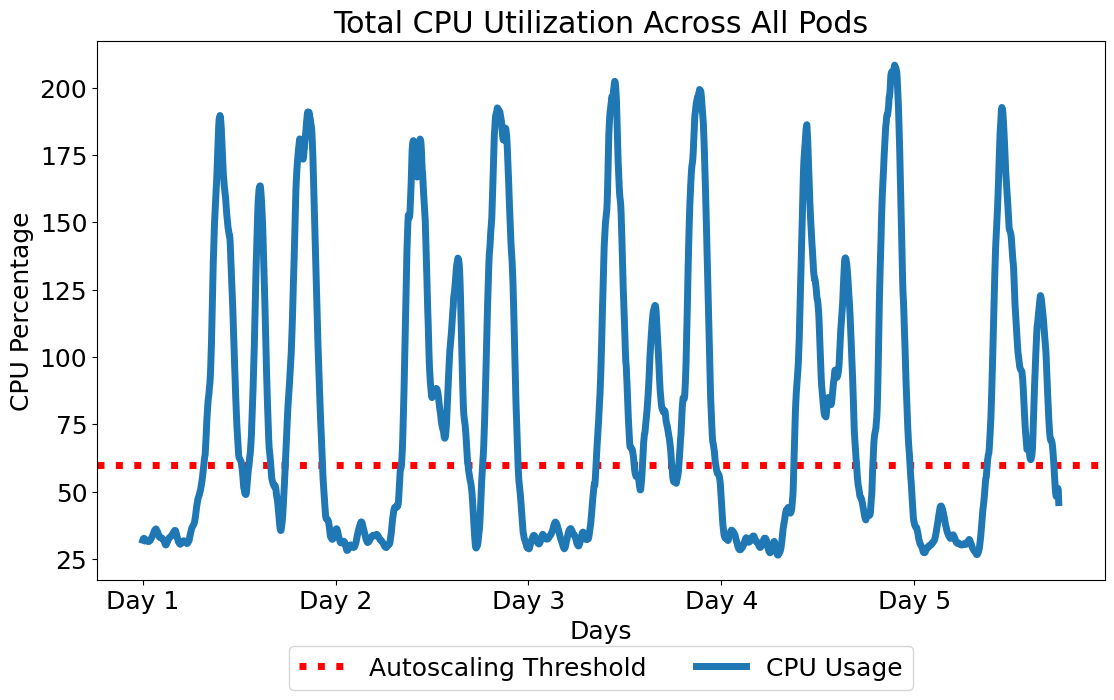
\includegraphics[width=0.6\linewidth]{Figures/POST-Total-CPU.pdf}
\end{figure}
\end{comment}

\begin{center}
\begin{minipage}{\linewidth}
    \captionof{figure}{Total CPU utilization for \textit{compose-post-service}}
    \label{fig:exp2-workload}
    \begin{tikzpicture}
        \begin{axis}[
            height=0.4\linewidth,
            width=\linewidth,
            xmin=0,
            xmax=2460,  % Make xmax 150 above the final xtick
            ymin=0,
            ymajorgrids=true,
            yminorgrids=true,
            xmajorgrids=true,
            xminorgrids=true,
            grid style=dashed,
            xlabel={Time (Days)},
            ylabel={CPU Usage (\%)},
            legend style={at={(0.5,-0.3)},anchor=north,legend columns=-1},
            xticklabels={Day 1, Day 2, Day 3, Day 4, Day 5},
            xtick={580, 1050, 1510, 1970, 2370},
            ytick={0, 60, 120, 180, 240}
        ]
            \addplot+[RoyalBlue, mark=none] table [x=xtick, y=value, col sep=comma] {Data/POST-Total-CPU.csv};
            \draw[red, thick, dashed] (axis cs:0, 60) -- (axis cs:2460, 60);
            \legend{CPU Usage}
            \addlegendimage{line width=0.3mm, dashed, color=red}
            \addlegendentry{Autoscaling Threshold}
        \end{axis}
    \end{tikzpicture}
\end{minipage}
\end{center}

While the SELECT statement used underneath the GET request was a fairly quick operation, the INSERT and UPDATE statements may take significantly longer, due to the idempotent nature of the database \cite{lutteroth2009database}. The social network will ensure that user posts are in the correct order, and perform other background checks before committing the data. Due to this, the connections on the \textit{compose-post-service} can remain open for a significantly longer amount of time, resulting in far more resources being used. Figure \ref{fig:exp2-workload} shows this in action. The algorithm was generated for a total of 5 days, similar to the first experiment. Even though the workload generation algorithm was sending the same amount of POST requests as it did GET requests, approximately \num[group-separator={,}]{2550000} requests in total, the total CPU workload in the second experiment peaked at approximately 175\%, and at some points even reached 200\% of the total CPU resources assigned to a unitary deployment pod. This varied per day in a realistic manner similar to what could commonly be seen in social networks.\par

To resolve this CPU bottleneck, the auto-scaling threshold was set to 60\% of the CPU workload. In addition, the SLA latency threshold was set to the flexible threshold of 1000 milliseconds. Using these configurations, the three baseline algorithms along with the proposed hybrid autoscaler was tested.\par

\section{Evaluation of Request Latency}
\label{sec:ch6-request-latency-eval}

\subsection {Default Kubernetes Autoscaler Baseline}
\label{subsec:ch6-default-algo}

\begin{comment}
\begin{figure}[htb]
    \centering
    \caption{Kubernetes Default Autoscaler Latency For \textit{home-timeline-service}}
    \label{fig:exp1-default-k8s}
    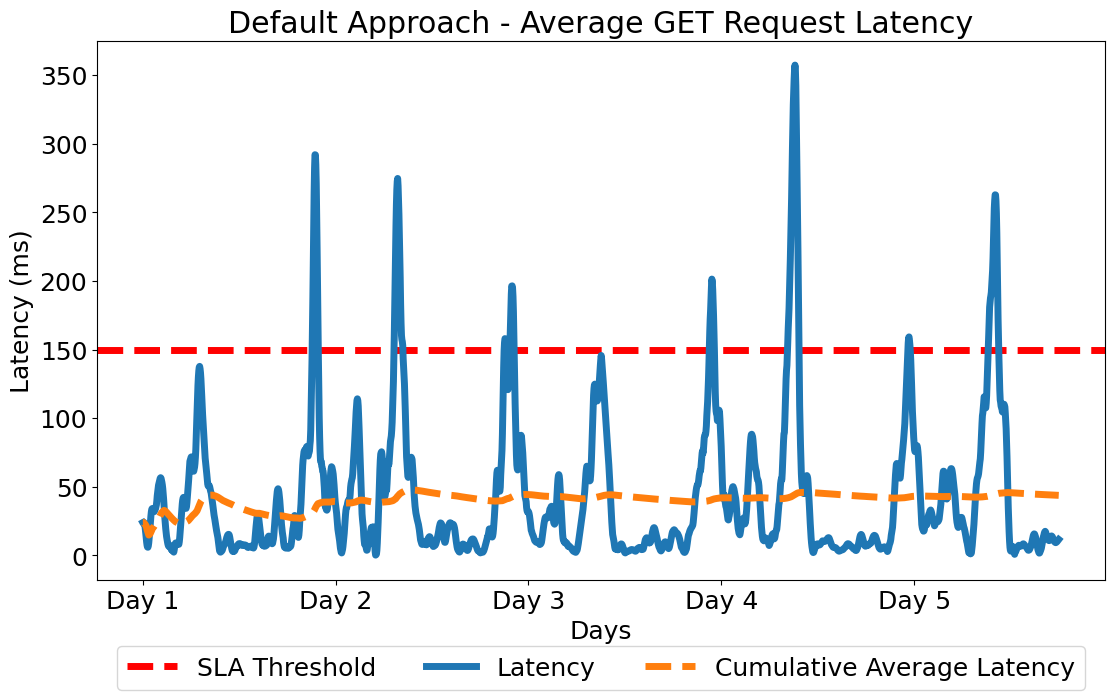
\includegraphics[width=0.6\linewidth]{Figures/Home-Timeline-Default-Latency.pdf}
\end{figure}
\end{comment}

\begin{center}
\begin{minipage}{\linewidth}
    \captionof{figure}{Kubernetes default sutoscaler latency for \textit{home-timeline-service}}
    \label{fig:exp1-default-k8s}
    \begin{tikzpicture}
        \begin{axis}[
            height=0.4\linewidth,
            width=\linewidth,
            xmin=0,
            xmax=2460,  % Make xmax 150 above the final xtick
            ymin=0,
            ymajorgrids=true,
            yminorgrids=true,
            xmajorgrids=true,
            xminorgrids=true,
            grid style=dashed,
            xlabel={Time (Days)},
            ylabel={Latency (ms)},
            legend style={at={(0.5,-0.3)},anchor=north,legend columns=-1},
            xticklabels={Day 1, Day 2, Day 3, Day 4, Day 5},
            xtick={570, 1030, 1510, 1950, 2370},
            ytick={0, 75, 150, 225, 300, 375}
        ]
            \addplot+[RoyalBlue, mark=none] table [x=xtick, y=value, col sep=comma] {Data/Home-Timeline-Default-Latency-CPU.csv};
            \addplot+[OliveGreen, mark=none] table [x=xtick, y=value, col sep=comma] {Data/Home-Timeline-Default-Latency-AVG.csv};
            \draw[red, thick, dashed] (axis cs:0, 150) -- (axis cs:2460, 150);
            \legend{Latency, Cumulative Average Latency}
            \addlegendimage{line width=0.3mm, dashed, color=red}
            \addlegendentry{SLA Threshold}
        \end{axis}
    \end{tikzpicture}
\end{minipage}
\end{center}

For both the workloads discussed above, a near 100\% CPU utilization on a solitary deployment pod would lead to significant delays. This can be seen when using the default Kubernetes Horizontal Pod Autoscaler in the first experiment, as depicted in figure \ref{fig:exp1-default-k8s}. The autoscaler was merely a primitive reactive implementation with no knowledge of which edge nodes were experiencing heavy traffic, and which ones were not. Thus, it blindly assigned pods to the nodes in a round-robin manner. Additionally, the autoscaler required a significant amount of time to register the new pods to the Kubernetes control plane, thus falling victim to the cold start problem. This results in significant latency spikes before the resources are adjusted. In the figure, it can be seen that the latency exceeds 300 milliseconds at some points, which would be significantly large enough to degrade the user experience. Additionally, by the end of the fifth day of testing, the cumulative average latency of the social-network was nearly 50 milliseconds.\par

\begin{comment}
\begin{figure}[htb]
    \centering
    \caption{Kubernetes Default Autoscaler Latency For \textit{compose-post-service}}
    \label{fig:exp2-default-k8s}
    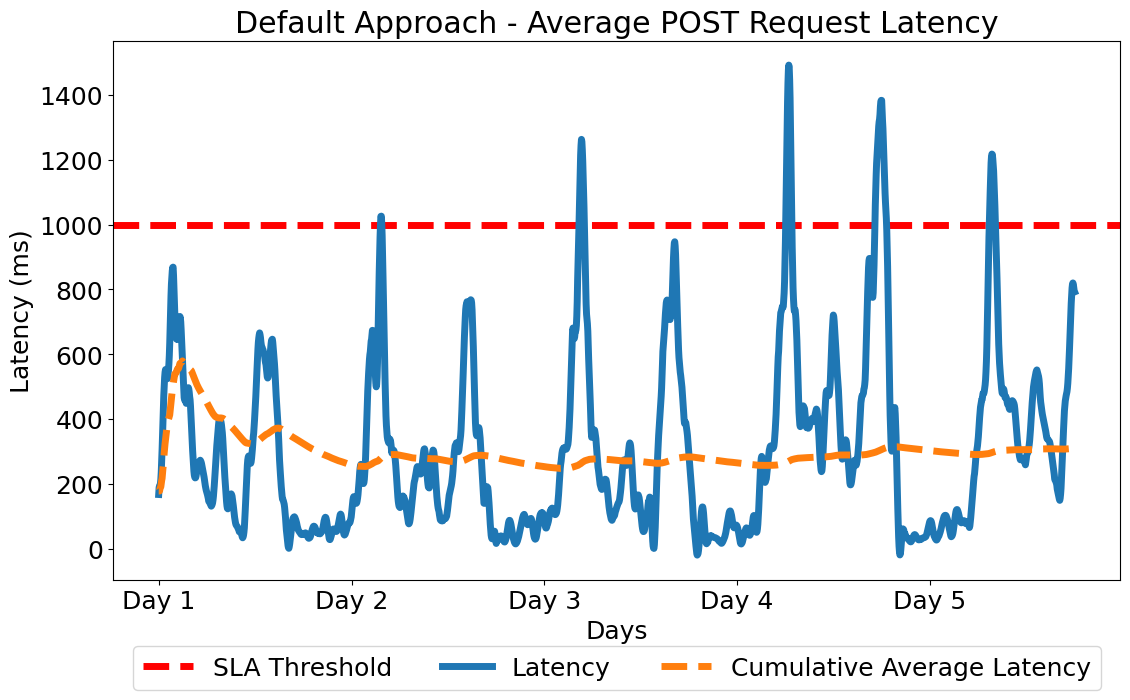
\includegraphics[width=0.6\linewidth]{Figures/Compose-Post-Default-Latency.pdf}
\end{figure}
\end{comment}

\begin{center}
\begin{minipage}{\linewidth}
    \captionof{figure}{Kubernetes default autoscaler latency for \textit{compose-post-service}}
    \label{fig:exp2-default-k8s}
    \begin{tikzpicture}
        \begin{axis}[
            height=0.4\linewidth,
            width=\linewidth,
            xmin=0,
            xmax=2460,  % Make xmax 150 above the final xtick
            ymin=0,
            ymajorgrids=true,
            yminorgrids=true,
            xmajorgrids=true,
            xminorgrids=true,
            grid style=dashed,
            xlabel={Time (Days)},
            ylabel={Latency (ms)},
            legend style={at={(0.5,-0.3)},anchor=north,legend columns=-1},
            xticklabels={Day 1, Day 2, Day 3, Day 4, Day 5},
            xtick={580, 1050, 1510, 1970, 2370}
        ]
            \addplot+[RoyalBlue, mark=none] table [x=xtick, y=value, col sep=comma] {Data/Compose-Post-Default-Latency-CPU.csv};
            \addplot+[OliveGreen, mark=none] table [x=xtick, y=value, col sep=comma] {Data/Compose-Post-Default-Latency-AVG.csv};
            \draw[red, thick, dashed] (axis cs:0, 1000) -- (axis cs:2460, 1000);
            \legend{Latency, Cumulative Average Latency}
            \addlegendimage{line width=0.3mm, dashed, color=red}
            \addlegendentry{SLA Threshold}
        \end{axis}
    \end{tikzpicture}
\end{minipage}
\end{center}

Similar to the results in the first experiment, the shortcomings of this auto-scaling approach were exposed even more so by the increased demands of the POST API workload in the second experiment. Figure \ref{fig:exp2-default-k8s} shows the latency metrics of the autoscaler. During the daily workload spikes, the autoscaler would regularly breach the 1000 millisecond threshold, with values peaking at almost 1450 milliseconds. This is more than 45\% above the allowed threshold, which would cause general system instability. Furthermore, the average latency of the autoscaler hovered at around the 400-millisecond mark throughout the experiment, which was quite a high value when taking into account the large periods of non-peak workload in the test.\par

Upon further investigation, it was discovered that the high latency was caused due to three issues. One was the cold start problem, which added a constant latency to the non-proactive algorithms which could not be solved by any reactive solutions. The second one was the avalanche effect which was caused by resources not being available in a timely manner, and was related to the cold start. Before the Kubernetes control plane could register all resources, the \textit{compose-post-service} deployment may have had a CPU utilization at or near 100\%. When this happened, the deployment already had all available resources being utilized to open connections, this caused additional connection requests to be dropped. The user does not see this happen and instead waits the default 60 seconds before displaying a ``time-out'' message. This 60 seconds was taken into account when measuring the latency and was what drove up the latency to such an extent. Finally, the Kubernetes default autoscaler had no information on which edge nodes were receiving the most number of requests. It only saw CPU utilization metrics as a totality. As a result of this, it scheduled new resources in a round-robin manner, meaning that some deployment pods received a lot of requests, while others may have received none. This uneven distribution of requests to the resources also drove up latency.\par

Based on these experimental results which showed that connections were being dropped, it meant that the social network was becoming unavailable at certain points in time during the day. This happening during peak hours was especially critical and violated SLA constraints. Due to this, the default Kubernetes autoscaler could not be considered viable for auto-scaling an edge deployment.

\subsection {Reactive THPA Autoscaler Baseline}
\label{subsec:ch6-reactive-algo}

\begin{comment}
\begin{figure}[htb]
    \centering
    \caption{THPA Reactive Autoscaler Latency For \textit{home-timeline-service}}
    \label{fig:exp1-reactive-k8s}
    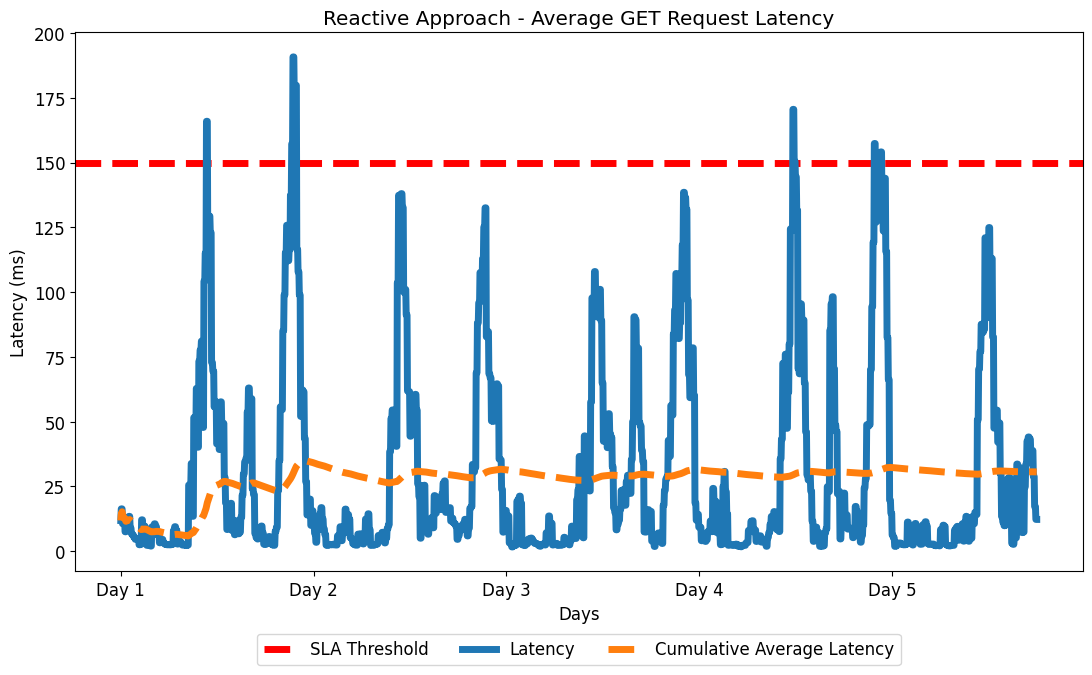
\includegraphics[width=0.6\linewidth]{Figures/Home-Timeline-Reactive-Latency.pdf}
\end{figure}
\end{comment}

\begin{center}
\begin{minipage}{\linewidth}
    \captionof{figure}{THPA reactive autoscaler latency for \textit{home-timeline-service}}
    \label{fig:exp1-reactive-k8s}
    \begin{tikzpicture}
        \begin{axis}[
            height=0.4\linewidth,
            width=\linewidth,
            xmin=0,
            xmax=2460,  % Make xmax 150 above the final xtick
            ymin=0,
            ymajorgrids=true,
            yminorgrids=true,
            xmajorgrids=true,
            xminorgrids=true,
            grid style=dashed,
            xlabel={Time (Days)},
            ylabel={Latency (ms)},
            legend style={at={(0.5,-0.3)},anchor=north,legend columns=-1},
            xticklabels={Day 1, Day 2, Day 3, Day 4, Day 5},
            xtick={570, 1030, 1510, 1950, 2370}
        ]
            \addplot+[RoyalBlue, mark=none] table [x=xtick, y=value, col sep=comma] {Data/Home-Timeline-Reactive-Latency-CPU.csv};
            \addplot+[OliveGreen, mark=none] table [x=xtick, y=value, col sep=comma] {Data/Home-Timeline-Reactive-Latency-AVG.csv};
            \draw[red, thick, dashed] (axis cs:0, 150) -- (axis cs:2460, 150);
            \legend{Latency, Cumulative Average Latency}
            \addlegendimage{line width=0.3mm, dashed, color=red}
            \addlegendentry{SLA Threshold}
        \end{axis}
    \end{tikzpicture}
\end{minipage}
\end{center}

Unlike the default Kubernetes autoscaler, THPA kept track of which edge node was receiving a significant number of requests and assigned pods to the nodes accordingly. This strategy resulted in a significantly improved latency graph for the first experiment, as can be seen in Figure \ref{fig:exp1-reactive-k8s}.\par

While the algorithm still suffered from the cold start problem, the more intelligent assignment of resources resulted in fewer availability issues, ensuring that the latency spikes that were seen were not as drastic as the ones in the default implementation. However, due to the cold start problem, the SLA threshold of 150ms was still regularly breached, resulting in several violations and degraded the user experience. However these breaches never exceeded the 200ms mark, and thus the drop in user experience quality was not as noticeable as the approach using the default Kubernetes baseline. Furthermore, the average latency over the experimental time frame was lower than what was seen in the default implementation, hovering at around 25-30 milliseconds.\par

\begin{comment}
\begin{figure}[htb]
    \centering
    \caption{THPA Reactive Autoscaler Latency For \textit{compose-post-service}}
    \label{fig:exp2-reactive-k8s}
    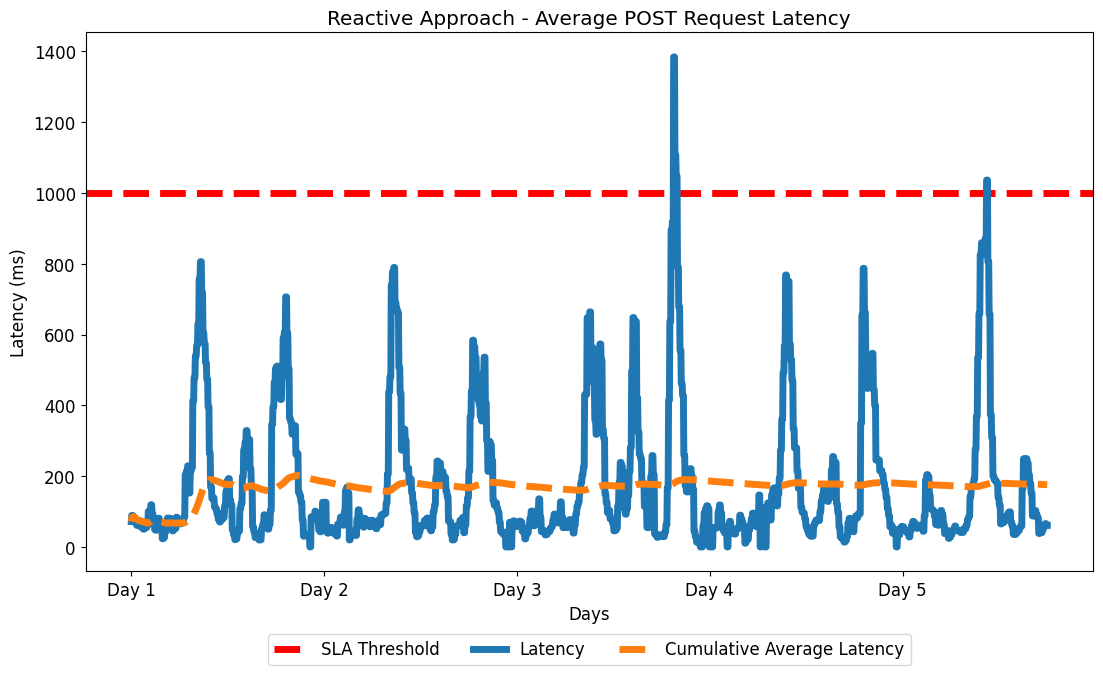
\includegraphics[width=0.6\linewidth]{Figures/Compose-Post-Reactive-Latency.pdf}
\end{figure}
\end{comment}

\begin{center}
\begin{minipage}{\linewidth}
    \captionof{figure}{THPA reactive autoscaler latency for \textit{compose-post-service}}
    \label{fig:exp2-reactive-k8s}
    \begin{tikzpicture}
        \begin{axis}[
            height=0.4\linewidth,
            width=\linewidth,
            xmin=0,
            xmax=2460,  % Make xmax 150 above the final xtick
            ymin=0,
            ymajorgrids=true,
            yminorgrids=true,
            xmajorgrids=true,
            xminorgrids=true,
            grid style=dashed,
            xlabel={Time (Days)},
            ylabel={Latency (ms)},
            legend style={at={(0.5,-0.3)},anchor=north,legend columns=-1},
            xticklabels={Day 1, Day 2, Day 3, Day 4, Day 5},
            xtick={580, 1050, 1510, 1970, 2370}
        ]
            \addplot+[RoyalBlue, mark=none] table [x=xtick, y=value, col sep=comma] {Data/Compose-Post-Reactive-Latency-CPU.csv};
            \addplot+[OliveGreen, mark=none] table [x=xtick, y=value, col sep=comma] {Data/Compose-Post-Reactive-Latency-AVG.csv};
            \draw[red, thick, dashed] (axis cs:0, 1000) -- (axis cs:2460, 1000);
            \legend{Latency, Cumulative Average Latency}
            \addlegendimage{line width=0.3mm, dashed, color=red}
            \addlegendentry{SLA Threshold}
        \end{axis}
    \end{tikzpicture}
\end{minipage}
\end{center}

Figure \ref{fig:exp2-reactive-k8s} shows how the THPA algorithm performed on the POST API workload for the second experiment. As expected, the request-aware architecture of this autoscaler allowed it to eliminate the issues with dropped requests seen in the Kubernetes autoscaler implementation. This was due to the autoscaler assigning resource pods to the edge nodes which were experiencing a high number of POST requests. This ensured that on average, the latency values were kept lower. Furthermore, the avalanche effect seen above was somewhat mitigated due to the more intelligent resource deployment model.\par

However, the cold start problem was not eliminated, which caused spikes in the latency when the autoscaler could not handle assigning resources in time. While this was less common in this implementation than in the default one, it nevertheless resulted in latency spiking above the SLA threshold for lengthy amounts of time on multiple occasions. On one occasion, the latency nearly hit 1400 milliseconds for several minutes before coming back down when the resource registration was completed.\par

These issues were not as severe as the ones seen in the default autoscaler however, and would not cause complete system unavailability. Furthermore, the cumulative average latency throughout the testing period was substantially lower than the default Kubernetes baseline, averaging at around 200 milliseconds. Despite this, SLA agreements were still being violated regularly, and thus while the autoscaler could be considered a suitable algorithm for native cloud deployments, it was deemed unsuitable for edge deployments with SLA constraints.\par

\subsection {Proactive PPA Autoscaler Baseline}
\label{subsec:ch6-proactive-algo}

Unlike the previous two baseline algorithms, the Proactive Pod Autoscaler algorithm attempted to predict the workload before it was requested, thus eliminating the cold start issue. In ideal conditions, this would result in the SLA threshold not being violated, and it being a viable solution for edge paradigms. However, experimental results showed otherwise.\par

\begin{comment}
\begin{figure}[htb]
    \centering
    \caption{PPA Proactive Autoscaler Latency For \textit{home-timeline-service}}
    \label{fig:exp1-proactive-k8s}
    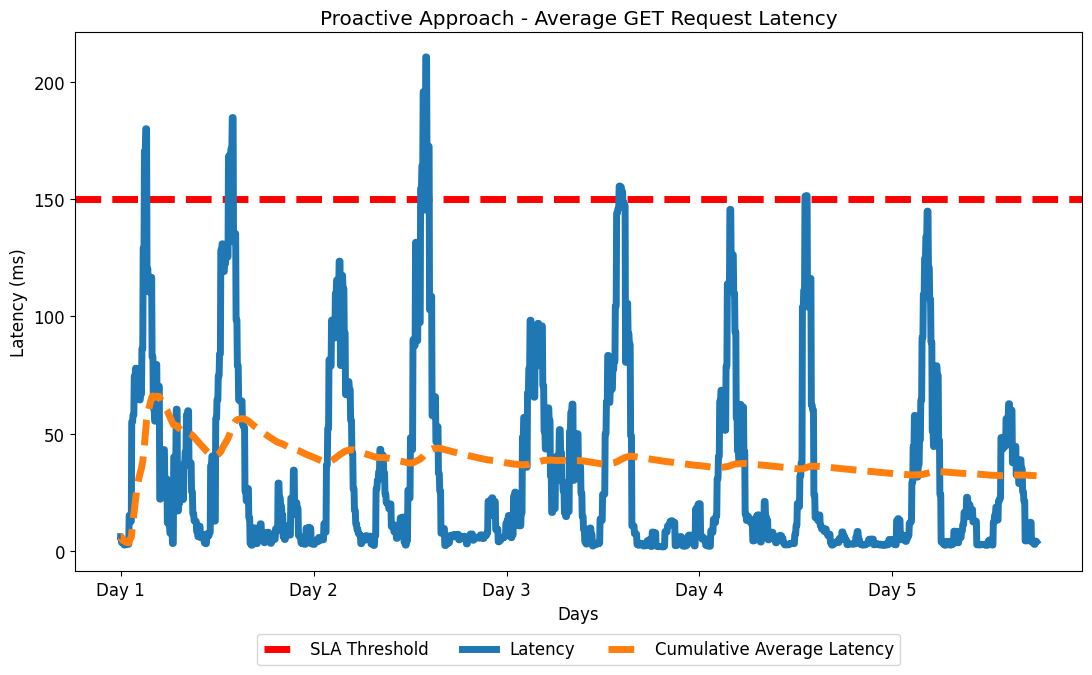
\includegraphics[width=0.6\linewidth]{Figures/Home-Timeline-Proactive-Latency.pdf}
\end{figure}
\end{comment}

\begin{center}
\begin{minipage}{\linewidth}
    \captionof{figure}{PPA proactive autoscaler latency for \textit{home-timeline-service}}
    \label{fig:exp1-proactive-k8s}
    \begin{tikzpicture}
        \begin{axis}[
            height=0.4\linewidth,
            width=\linewidth,
            xmin=0,
            xmax=2460,  % Make xmax 150 above the final xtick
            ymin=0,
            ymajorgrids=true,
            yminorgrids=true,
            xmajorgrids=true,
            xminorgrids=true,
            grid style=dashed,
            xlabel={Time (Days)},
            ylabel={Latency (ms)},
            legend style={at={(0.5,-0.3)},anchor=north,legend columns=-1},
            xticklabels={Day 1, Day 2, Day 3, Day 4, Day 5},
            xtick={570, 1030, 1510, 1950, 2370},
            ytick={0, 75, 150, 225, 300, 375}
        ]
            \addplot+[RoyalBlue, mark=none] table [x=xtick, y=value, col sep=comma] {Data/Home-Timeline-Proactive-Latency-CPU.csv};
            \addplot+[OliveGreen, mark=none] table [x=xtick, y=value, col sep=comma] {Data/Home-Timeline-Proactive-Latency-AVG.csv};
            \draw[red, thick, dashed] (axis cs:0, 150) -- (axis cs:2460, 150);
            \legend{Latency, Cumulative Average Latency}
            \addlegendimage{line width=0.3mm, dashed, color=red}
            \addlegendentry{SLA Threshold}
        \end{axis}
    \end{tikzpicture}
\end{minipage}
\end{center}

Because the autoscaler was purely proactive, it must be a deep LSTM model with several layers and large training epochs. This deep model took more than 50 minutes to properly train and validate for it to predict 24 hours of data, similar to the length of data that our proposed hybrid solution predicted. This is due to the edge architecture's lack of resources and storage compared to the cloud layer. Figure \ref{fig:exp1-proactive-k8s} shows this in action for the first experiment. Initially, it was observed that the latency continually spiked, causing a large amount of SLA violations, more than what the reactive autoscaler caused. However, after a few days of training, the rolling update structure of the LSTM weights took over, reducing the training time by taking advantage of the early stopping callback in the LSTM model, and managing to stabilize the latency. However, this effect did not always manage to stem the latency overflow, as was shown when the same algorithm was tested using the POST API in section \ref{subsec:ch6-proactive-algo}.

While the SLA violations were not as severe as the ones seen in the Default autoscaler baseline, they were comparatively greater than the reactive approach, with the latency exceeding 200 milliseconds for several minutes during the day, which would cause a noticeable delay. The average latency was almost as large as what was seen in the default autoscaler baseline, approaching 50 milliseconds due to the issues inherent in attempting to forecast the entire time-series data curve.\par

\begin{comment}
\begin{figure}[htb]
    \centering
    \caption{PPA Proactive Autoscaler Latency For \textit{compose-post-service}}
    \label{fig:exp2-proactive-k8s}
    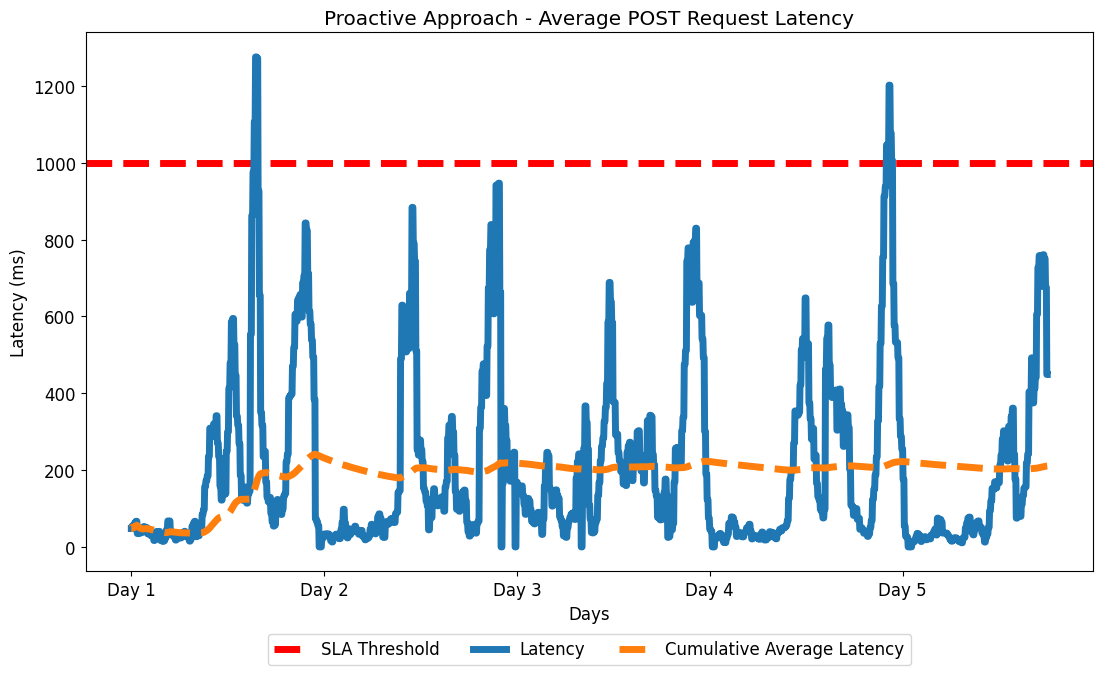
\includegraphics[width=0.6\linewidth]{Figures/Compose-Post-Proactive-Latency.pdf}
\end{figure}
\end{comment}

\begin{center}
\begin{minipage}{\linewidth}
    \captionof{figure}{PPA proactive autoscaler latency for \textit{compose-post-service}}
    \label{fig:exp2-proactive-k8s}
    \begin{tikzpicture}
        \begin{axis}[
            height=0.4\linewidth,
            width=\linewidth,
            xmin=0,
            xmax=2460,  % Make xmax 150 above the final xtick
            ymin=0,
            ymajorgrids=true,
            yminorgrids=true,
            xmajorgrids=true,
            xminorgrids=true,
            grid style=dashed,
            xlabel={Time (Days)},
            ylabel={Latency (ms)},
            legend style={at={(0.5,-0.3)},anchor=north,legend columns=-1},
            xticklabels={Day 1, Day 2, Day 3, Day 4, Day 5},
            xtick={580, 1050, 1510, 1970, 2370}
        ]
            \addplot+[RoyalBlue, mark=none] table [x=xtick, y=value, col sep=comma] {Data/Compose-Post-Proactive-Latency-CPU.csv};
            \addplot+[OliveGreen, mark=none] table [x=xtick, y=value, col sep=comma] {Data/Compose-Post-Proactive-Latency-AVG.csv};
            \draw[red, thick, dashed] (axis cs:0, 1000) -- (axis cs:2460, 1000);
            \legend{Latency, Cumulative Average Latency}
            \addlegendimage{line width=0.3mm, dashed, color=red}
            \addlegendentry{SLA Threshold}
        \end{axis}
    \end{tikzpicture}
\end{minipage}
\end{center}

Figure \ref{fig:exp2-proactive-k8s} shows the full latency graph for the social network for the second experiment. As can be seen from the data, the latency initially spiked to above 1200 milliseconds, before stabilizing below the SLA threshold. However, one more spike occurred on the last day. Finally, the average latency of the autoscaler performed well, having a value of around 200 milliseconds which was similar to the reactive baseline.\par

Further investigations were conducted in an attempt to explain why these spikes occurred. It was deduced that the first latency spike occurred due to a shortage of training data. The LSTM used by the PPA architecture is extremely complex. Furthermore, apart from data normalization, no other data pre-processing was done such as passing it through the Savitsky-Golay smoothing algorithm. These issues make it more difficult for the forecaster to correctly predict data curves early on in its life cycle. This issue was resolved as more data was added to the training time-series input, however, after a certain point, a threshold was reached where the data was so large, it took a significantly large amount of time for the autoscaler to forecast the workload. This issue led to the latency spike on the final day leading to SLA violations, lasting for several minutes before the autoscaler corrected itself.\par

From these investigations, it can be seen that the proactive auto-scaling approach worked significantly better than the default Kubernetes autoscaler, but performed similarly to the reactive approach. While the social network POST requests were never dropped which would lead to complete system unavailability, the SLA constraints were nonetheless breached, due to the lack of edge layer resources and large training times for the proactive model. Due to issues such as this, the algorithm could not be deemed suitable for edge deployments that were reliant on SLA constraints.\par

\subsection {Proposed Hybrid Autoscaler}
\label{subsec:ch6-hybrid-algo}

\begin{comment}
\begin{figure}[htb]
    \centering
    \caption{Hybrid Autoscaler Latency For \textit{home-timeline-service}}
    \label{fig:exp1-hybrid-k8s}
    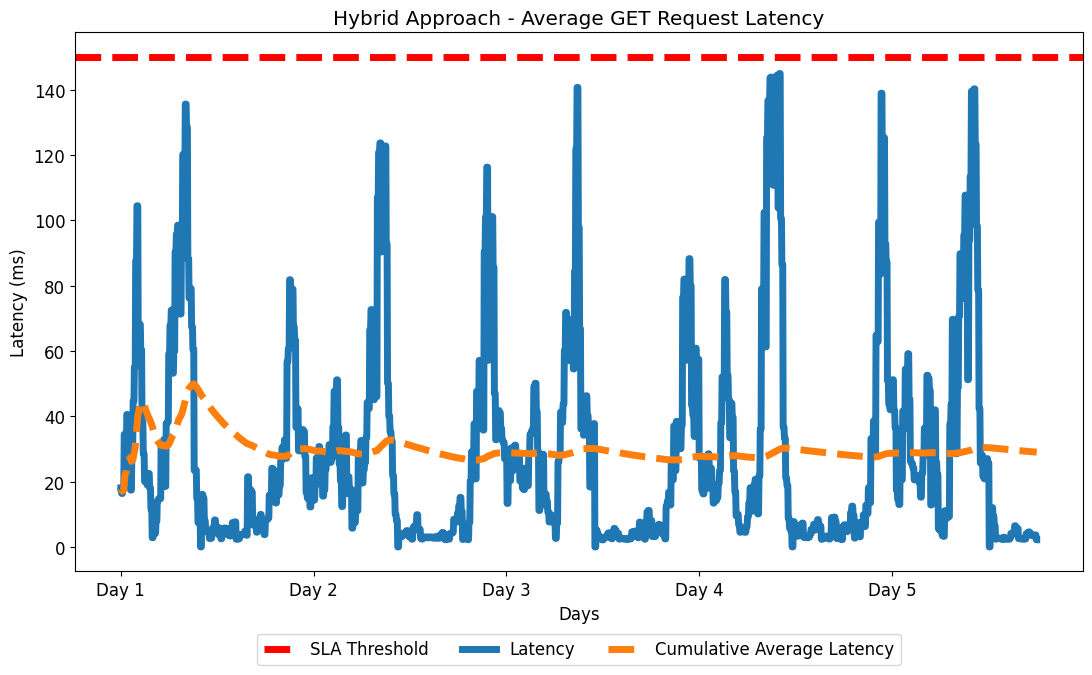
\includegraphics[width=0.6\linewidth]{Figures/Home-Timeline-Hybrid-Latency.pdf}
\end{figure}
\end{comment}

\begin{center}
\begin{minipage}{\linewidth}
    \captionof{figure}{Hybrid autoscaler latency for \textit{home-timeline-service}}
    \label{fig:exp1-hybrid-k8s}
    \begin{tikzpicture}
        \begin{axis}[
            height=0.4\linewidth,
            width=\linewidth,
            xmin=0,
            xmax=2460,  % Make xmax 150 above the final xtick
            ymin=0,
            ymajorgrids=true,
            yminorgrids=true,
            xmajorgrids=true,
            xminorgrids=true,
            grid style=dashed,
            xlabel={Time (Days)},
            ylabel={Latency (ms)},
            legend style={at={(0.5,-0.3)},anchor=north,legend columns=-1},
            xticklabels={Day 1, Day 2, Day 3, Day 4, Day 5},
            xtick={570, 1030, 1510, 1950, 2370}
        ]
            \addplot+[RoyalBlue, mark=none] table [x=xtick, y=value, col sep=comma] {Data/Home-Timeline-Hybrid-Latency-CPU.csv};
            \addplot+[OliveGreen, mark=none] table [x=xtick, y=value, col sep=comma] {Data/Home-Timeline-Hybrid-Latency-AVG.csv};
            \draw[red, thick, dashed] (axis cs:0, 150) -- (axis cs:2460, 150);
            \legend{Latency, Cumulative Average Latency}
            \addlegendimage{line width=0.3mm, dashed, color=red}
            \addlegendentry{SLA Threshold}
        \end{axis}
    \end{tikzpicture}
\end{minipage}
\end{center}

Finally, with the baselines being established in a default, reactive, and proactive approach, the hybrid algorithm was tested on the five days of generated workload. This approach demonstrated how it could mitigate the issues seen in both reactive and proactive auto-scaling approaches. The autoscaler was extremely lightweight, and easy to configure since there was no hyper-parameter tuning required. Building on top of this lightweight, the proactive forecaster was able to forecast the beginning of the workload spike accurately, thus leading to it eliminating the issue of a cold start. The forecaster could not accurately predict the middle and end of the daily workloads, however, this was not an issue, since the reactive algorithm was capable of taking over the auto-scaling process and maintaining the necessary resources to avoid SLA violations. Figure \ref{fig:exp1-hybrid-k8s} shows the complete latency graph for the GET API experiment.\par

From the graph, it is clear that for the GET request experiment, no SLA violations were present for the duration of the five-day workload. Thus, in this case, the autoscaler controller did not intervene in the LSTM training procedure and modify the hyper-parameters of the forecaster. The average latency experienced by the social network was also comparatively low, achieving results similar to the THPA reactive implementation with the value hovering at around 30 milliseconds. This performance was a significant improvement over the baseline algorithms and demonstrated the efficacy of such a model in an edge architecture deployment.\par

\begin{comment}
\begin{figure}[htb]
    \centering
    \caption{Hybrid Autoscaler Latency For \textit{compose-post-service}}
    \label{fig:exp2-hybrid-k8s}
    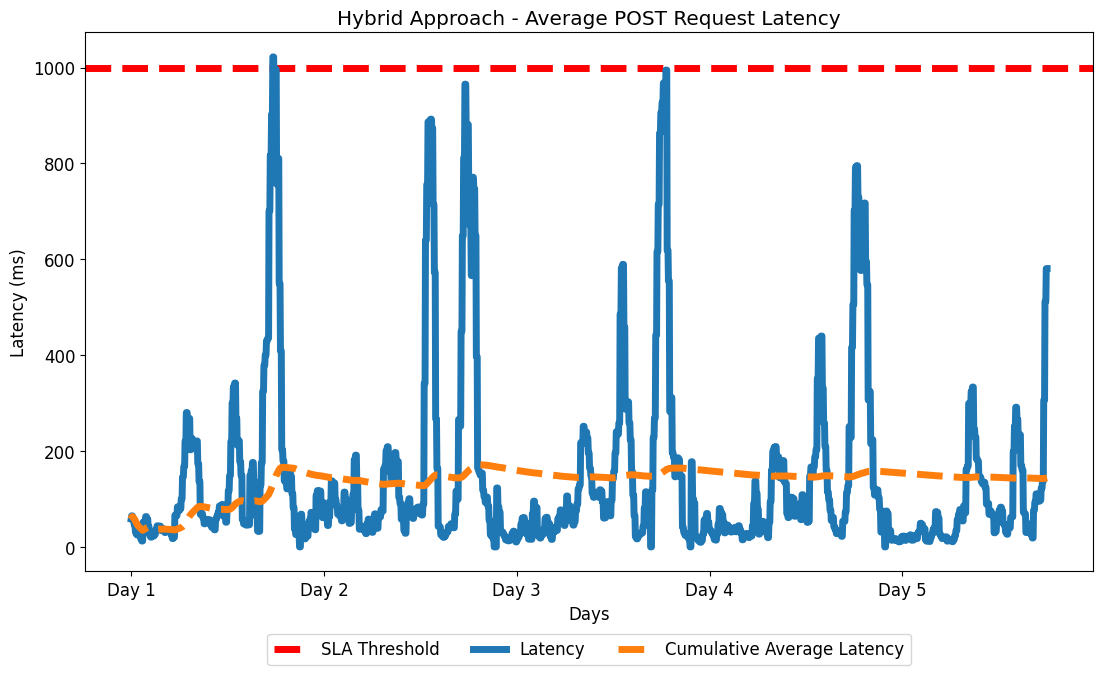
\includegraphics[width=0.6\linewidth]{Figures/Compose-Post-Hybrid-Latency.pdf}
\end{figure}
\end{comment}

\begin{center}
\begin{minipage}{\linewidth}
    \captionof{figure}{Hybrid autoscaler latency for \textit{compose-post-service}}
    \label{fig:exp2-hybrid-k8s}
    \begin{tikzpicture}
        \begin{axis}[
            height=0.4\linewidth,
            width=\linewidth,
            xmin=0,
            xmax=2460,  % Make xmax 150 above the final xtick
            ymin=0,
            ymajorgrids=true,
            yminorgrids=true,
            xmajorgrids=true,
            xminorgrids=true,
            grid style=dashed,
            xlabel={Time (Days)},
            ylabel={Latency (ms)},
            legend style={at={(0.5,-0.3)},anchor=north,legend columns=-1},
            xticklabels={Day 1, Day 2, Day 3, Day 4, Day 5},
            xtick={580, 1050, 1510, 1970, 2370}
        ]
            \addplot+[RoyalBlue, mark=none] table [x=xtick, y=value, col sep=comma] {Data/Compose-Post-Hybrid-Latency-CPU.csv};
            \addplot+[OliveGreen, mark=none] table [x=xtick, y=value, col sep=comma] {Data/Compose-Post-Hybrid-Latency-AVG.csv};
            \draw[red, thick, dashed] (axis cs:0, 1000) -- (axis cs:2460, 1000);
            \legend{Latency, Cumulative Average Latency}
            \addlegendimage{line width=0.3mm, dashed, color=red}
            \addlegendentry{SLA Threshold}
        \end{axis}
    \end{tikzpicture}
\end{minipage}
\end{center}

Figure \ref{fig:exp2-hybrid-k8s} shows the latency metrics for the five-day workload simulation period for the second POST API experiment. From the graph, it can be clearly seen that only one SLA violation took place on the first day. This was a result of the lack of training data causing an erroneous prediction, an issue faced by the proactive baseline algorithm as well. However, what set this algorithm apart from that baseline was that the reactive autoscaler subsystem was capable of taking over from the proactive subsystem and scaling the resources accordingly. Due to this, the SLA threshold was only breached slightly, peaking at around 1020 milliseconds.\par
After the SLA violation, the autoscaler controller deduced that the training process needed to be kick-started through hyper-parameter tuning. This was done in the next training cycle when the controller provided the forecaster new hyper-parameter values, and as a result, it can be seen that no SLA violations took place on the next day. As a result, the autoscaler controller resets the hyper-parameters to speed up the training process, and even though the latency approached 990 milliseconds on the third day, no further violations took place for the rest of the simulation. The average latency of the whole experiment was also kept below 200 milliseconds, performing slightly better than its reactive and proactive baseline counterparts, and significantly better than the default Kubernetes approach.\par

From these tests, it was clear that the hybrid approach had nearly eliminated the cold start problem very early on in the experiment. The initial difficulties in correctly forecasting the workload peaks were quickly resolved by the autoscaler controller's corrective instructions. All this was done with no user intervention, making the autoscaler extremely autonomous. Furthermore, the algorithm was capable of completing the training within a few minutes, allowing it to finish resource registration quickly. This meant that the CPU utilization of each pod on the nodes never exceeded 100\%, and thus no user API requests were dropped, allowing for full system availability.\par

Based on these results, it was experimentally demonstrated that the proposed hybrid autoscaler performed far better than the baseline algorithms, breaching the SLA threshold in a negligible amount while causing no system unavailability. Thus, the suitability of this hybrid approach for an edge deployment under SLA constraints was proven.

\section{Evaluation of CPU Workload Distribution}
\label{sec:ch6-cpu-workload-eval}

The distribution of CPU $workload$ across the deployment pods was another important metric to factor into the analysis. As a reminder, the goal of the autoscaler was to maximize deployment resources while minimizing deployment costs. Considering the equal importance to be given to both SLA latency and optimization costs as explained in section \ref{subsec:ch4-problem-formulation}, and with an autoscaler threshold being set at $\mathcal{A}$, ideally, the distributed workload should hover at $\frac{\mathcal{A}}{2}$. When this $workload$ distribution value approaches the value $\mathcal{A}$, it means that not enough pods are being deployed. This results in most if not all active pod resources in the deployment being utilized at full capacity, meaning new requests would need to be queued or even dropped, driving up latency. On the other hand, when $workload$ tends towards the value $0$, it means too many pods have been assigned to the deployment, and thus has been over-scaled. The returns when it comes to latency reduction for such a scaling scenario are extremely low, while the number of idle resource pods being active in the deployment is increasing significantly. This in turn increases the cost of running the underlying edge architecture, making this autoscaler an unprofitable alternative.\par

\begin{comment}
\begin{figure}[htb]
    \centering
    \caption{Autoscaler CPU Workload Distribution Comparison For \textit{home-timeline-service}}
    \label{fig:exp1-cpu-avg-dist}
    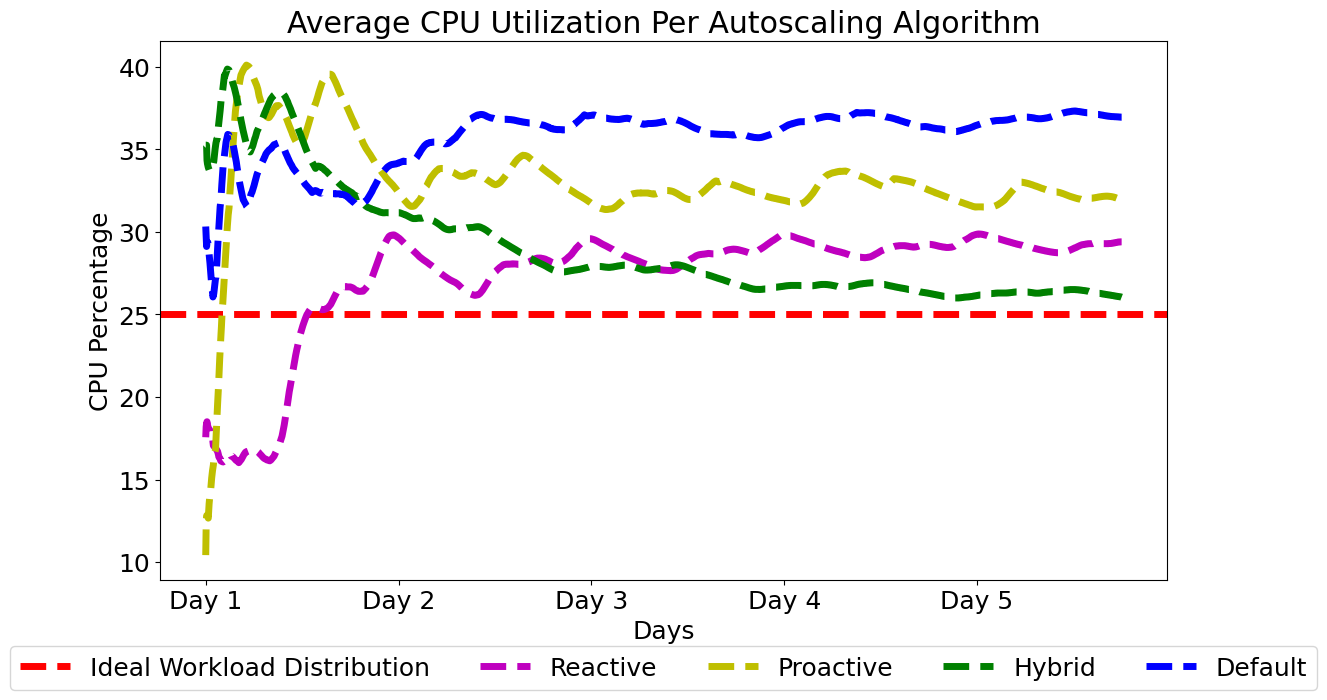
\includegraphics[width=0.6\linewidth]{Figures/Home-Timeline-CPU-Usage.pdf}
\end{figure}
\end{comment}

\begin{center}
\begin{minipage}{\linewidth}
    \captionof{figure}{Autoscaler CPU workload distribution for \textit{home-timeline-service}}
    \label{fig:exp1-cpu-avg-dist}
    \begin{tikzpicture}
        \begin{axis}[
            height=0.4\linewidth,
            width=\linewidth,
            xmin=0,
            xmax=2460,  % Make xmax 150 above the final xtick
            ymin=0,
            ymajorgrids=true,
            yminorgrids=true,
            xmajorgrids=true,
            xminorgrids=true,
            grid style=dashed,
            xlabel={Time (Days)},
            ylabel={CPU Usage (\%)},
            legend style={at={(0.5,-0.3)},anchor=north,legend columns=-1},
            xticklabels={Day 1, Day 2, Day 3, Day 4, Day 5},
            xtick={570, 1030, 1510, 1950, 2370},
            ytick={0, 20, 25, 40}
        ]
            \addplot+[RoyalBlue, mark=none] table [x=xtick, y=value, col sep=comma] {Data/Home-Timeline-CPU-Usage-Default.csv};
            \addplot+[Magenta, mark=none] table [x=xtick, y=value, col sep=comma] {Data/Home-Timeline-CPU-Usage-Reactive.csv};
            \addplot+[Apricot, mark=none] table [x=xtick, y=value, col sep=comma] {Data/Home-Timeline-CPU-Usage-Proactive.csv};
            \addplot+[OliveGreen, mark=none] table [x=xtick, y=value, col sep=comma] {Data/Home-Timeline-CPU-Usage-Hybrid.csv};
            \draw[red, thick, dashed] (axis cs:0, 25) -- (axis cs:2460, 25);
            \legend{Default, Reactive, Proactive, Hybrid}
            \addlegendimage{line width=0.3mm, dashed, color=red}
            \addlegendentry{Ideal CPU Usage}
        \end{axis}
    \end{tikzpicture}
\end{minipage}
\end{center}

For the first experiment, figure \ref{fig:exp1-cpu-avg-dist} shows the average CPU utilization $workload$ values of all the deployment pods for the three baseline algorithms and the proposed hybrid solution. As expected, the default Kubernetes horizontal pod autoscaler performs the worst, with the average utilization hovering around 35\%. The proactive forecaster has utilization of approximately 33\%, with it being held back by the forecaster's complexity and resource-intensive training. The reactive approach was the most lightweight autoscaler, and thus performed well with a CPU utilization of around 30\%. Finally, the hybrid autoscaler performed the best of the four compared algorithms, with the utilization of approximately 26\%.\par

In the second experiment with the heavier POST API, the auto-scaling threshold of the experiment $\mathcal{A}$ was set to 60\%. Thus the ideal distributed workload achieved by the autoscaler should be half of the threshold, as calculated in the first experiment. Hence, the distributed workload for this experiment should be $\frac{60}{2} = 30\%$

\begin{comment}
\begin{figure}[htb]
    \centering
    \caption{Autoscaler CPU Workload Distribution Comparison For \textit{compose-post-service}}
    \label{fig:exp2-cpu-avg-dist}
    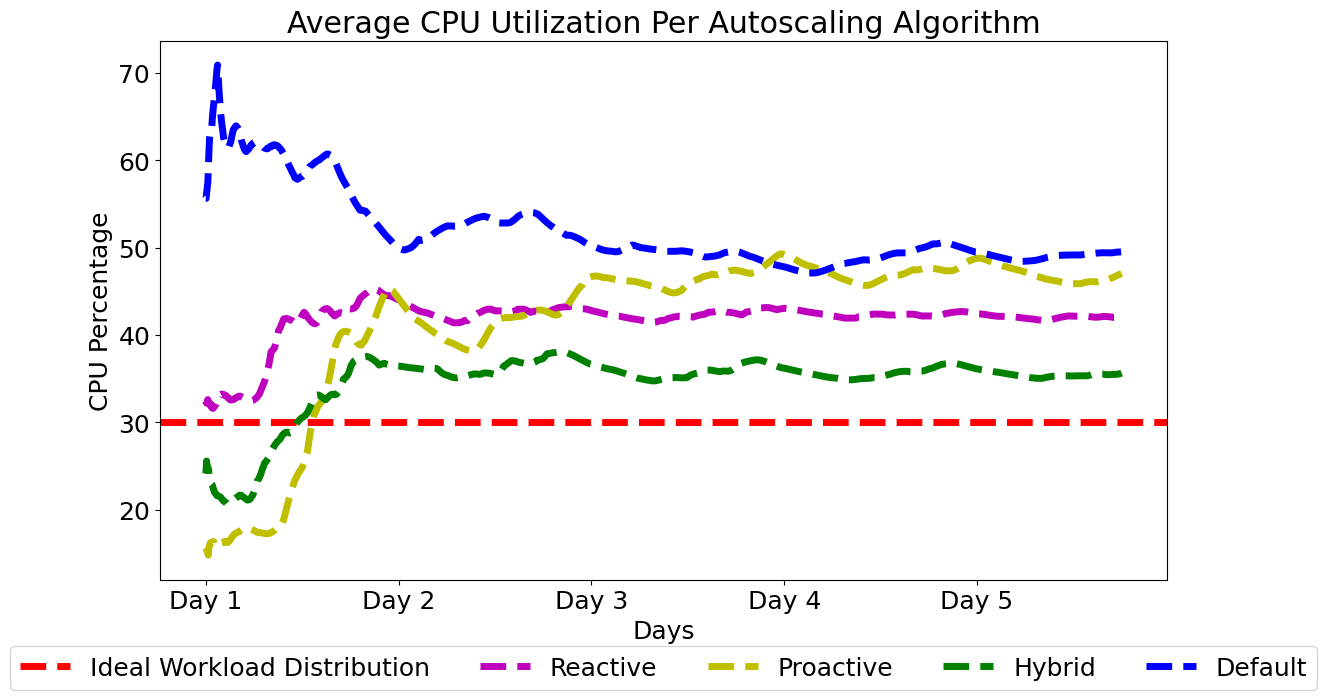
\includegraphics[width=0.6\linewidth]{Figures/Compose-Post-CPU-Usage.pdf}
\end{figure}
\end{comment}

\begin{center}
\begin{minipage}{\linewidth}
    \captionof{figure}{Autoscaler CPU workload distribution for \textit{compose-post-service}}
    \label{fig:exp2-cpu-avg-dist}
    \begin{tikzpicture}
        \begin{axis}[
            height=0.4\linewidth,
            width=\linewidth,
            xmin=0,
            xmax=2460,  % Make xmax 150 above the final xtick
            ymin=0,
            ymajorgrids=true,
            yminorgrids=true,
            xmajorgrids=true,
            xminorgrids=true,
            grid style=dashed,
            xlabel={Time (Days)},
            ylabel={CPU Usage (\%)},
            legend style={at={(0.5,-0.3)},anchor=north,legend columns=-1},
            xticklabels={Day 1, Day 2, Day 3, Day 4, Day 5},
            xtick={580, 1050, 1510, 1970, 2370},
            ytick={0, 15, 30, 45, 60, 75}
        ]
            \addplot+[RoyalBlue, mark=none] table [x=xtick, y=value, col sep=comma] {Data/Compose-Post-CPU-Usage-Default.csv};
            \addplot+[Magenta, mark=none] table [x=xtick, y=value, col sep=comma] {Data/Compose-Post-CPU-Usage-Reactive.csv};
            \addplot+[Apricot, mark=none] table [x=xtick, y=value, col sep=comma] {Data/Compose-Post-CPU-Usage-Proactive.csv};
            \addplot+[OliveGreen, mark=none] table [x=xtick, y=value, col sep=comma] {Data/Compose-Post-CPU-Usage-Hybrid.csv};
            \draw[red, thick, dashed] (axis cs:0, 30) -- (axis cs:2460, 30);
            \legend{Default, Reactive, Proactive, Hybrid}
            \addlegendimage{line width=0.3mm, dashed, color=red}
            \addlegendentry{Ideal CPU Usage}
        \end{axis}
    \end{tikzpicture}
\end{minipage}
\end{center}

Figure \ref{fig:exp2-cpu-avg-dist} shows the average CPU utilization of the pods for the second experiment, being scaled in the deployment by the three baseline algorithms, along with the proposed hybrid solution. As shown above in section \ref{subsec:ch6-default-algo}, the default Kubernetes autoscaler faced issues with system unavailability, with user requests being dropped. This was caused by high CPU usage on the pods, with this being demonstrated by the graph. The average utilization peaked at around 70\% before stabilizing at around 50\% for all the resource pods. However, it is important to note that these resources were not distributed equitably, and thus while some pods had close to 100\% utilization, others had near 0\%.\par

The baseline proactive PPA algorithm performed better than the default Kubernetes autoscaler. While its CPU utilization stabilized fairly quickly to a value of approximately 45\%, this was still far higher than the ideal distributed workload. This was most likely caused by the time it took for the algorithm to forecast data due to the complexity of the LSTM model, which resulted in resources lacking for certain periods of time.\par

The reactive THPA algorithm performed better than the proactive approach, with an average CPU utilization of approximately 42\%. This was achieved due to the intelligent placement of pods in the edge nodes through its traffic-aware algorithm. However, the autoscaler was still prone to the cold start problem, and thus there were several occasions where the CPU workload would peak before the appropriate resources could be assigned. Due to this, the average workload was still far higher than the ideal value.\par

Finally, it can be seen from the graph that the hybrid autoscaler performed better than all three of the baseline algorithms. Its proactive subsystem allowed it to nearly eliminate the cold start problem, while its short training times, and reactive subsystem, allowed the efficient placement of resource pods on the deployment. The average CPU workload quickly stabilized to approximately 35\%, which is far lower than the averages we have seen above for the baseline algorithms, and close to the ideal value of 30\%.\par

Through this comparison, it was clearly demonstrated that for multiple use cases, the hybrid autoscaler managed to scale resources in a manner that both mitigated SLA violations, while doing so in a manner that was both light-weight enough for edge deployments, and inexpensive too.\par

\section{Evaluation of SLA Violation Rates}
\label{sec:ch6-sla-violation-eval}

As demonstrated above, the hybrid autoscaler performed significantly better than the baseline approaches. However, this was only compared using the flexible SLA thresholds. As a reminder, this was the most lenient threshold possible. For a more thorough demonstration, the algorithms needed to be tested on the other possible latency thresholds.\par

To achieve this, all four algorithms were tested again on the moderate and strict SLA violation thresholds for the GET API, as displayed in table \ref{tab:experiment-sla-values}. The IoT workload generation algorithm was once again used to generate this, however, this time the workload was run for five days, but auto-scaling was performed only for the last two days. This was done to get the best possible results for all autoscalers regardless of training data length. This resulted in the SLA violation percentage for approximately \num[group-separator={,}]{1020000} GET requests.\par

\begin{comment}
\begin{figure}[htb]
    \centering
    \caption{SLA Violation Percentages For \textit{home-timeline-service}}
    \label{fig:exp1-sla-violation-bar}
    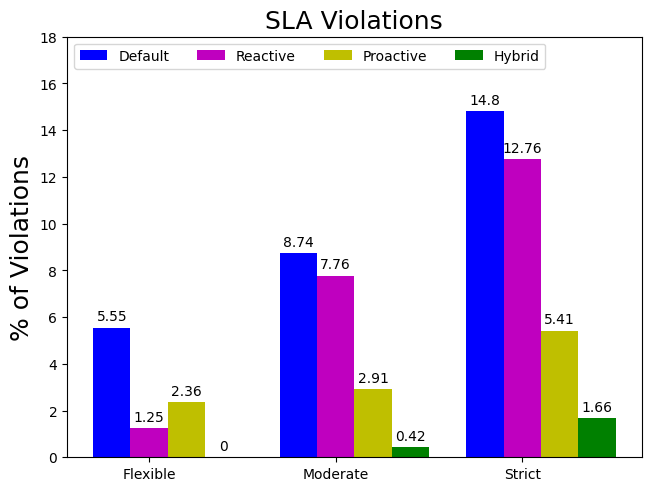
\includegraphics[width=0.6\linewidth]{Figures/Home-Timeline-SLA-Violations.pdf}
\end{figure}

\begin{center}
\begin{minipage}{\linewidth}
    \captionof{figure}{SLA Violation Percentages For \textit{home-timeline-service}}
    \label{fig:exp1-sla-violation-bar}
    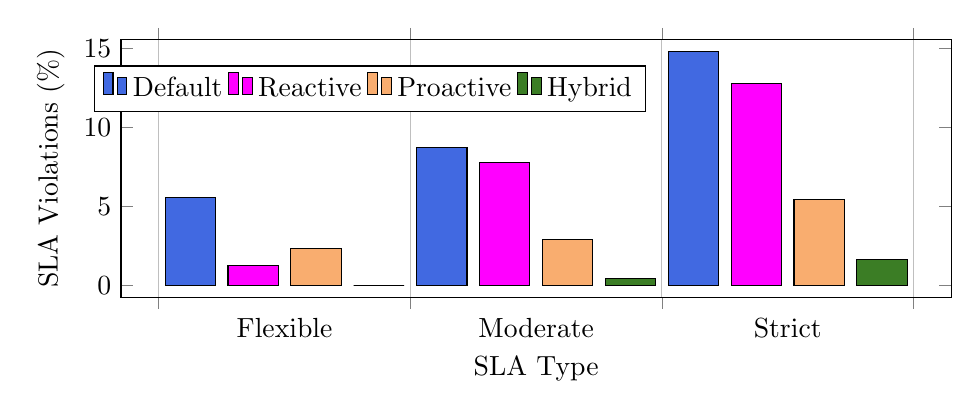
\begin{tikzpicture}
        \begin{axis}[
            height=0.4\linewidth,
            width=\linewidth,
            x tick label style={
                /pgf/number format/1000 sep=},
            ylabel=SLA Violations (\%),
            xlabel=SLA Type,
            enlargelimits=0.05,
            legend style={at={(0.3,0.9)},
            anchor=north,legend columns=-1},
            ybar interval=0.8,
            %symbolic x coords = {5,10,50,100,500,1000,DUMMY}
            xticklabels={Flexible, Moderate, Strict, DUMMY},
            xtick={5, 10, 15, 20}
        ]
        \addplot [fill = RoyalBlue]
        coordinates {(5,5.55) (10,8.74) (15,14.8) (20, 0)};
        \addplot [fill = Magenta]
        coordinates {(5,1.25) (10,7.76) (15,12.76) (20, 0)};
        \addplot [fill = Apricot]
        coordinates {(5,2.36) (10,2.91) (15,5.41) (20, 0)};
        \addplot [fill = OliveGreen]
        coordinates {(5,0) (10,0.42) (15,1.66) (20, 0)};
        \legend{Default, Reactive, Proactive, Hybrid}
        \end{axis}
    \end{tikzpicture}
\end{minipage}
\end{center}
\end{comment}

\begin{center}
\begin{minipage}{\linewidth}
    \captionof{figure}{SLA violation percentages for \textit{home-timeline-service}}
    \label{fig:exp1-sla-violation-bar}
    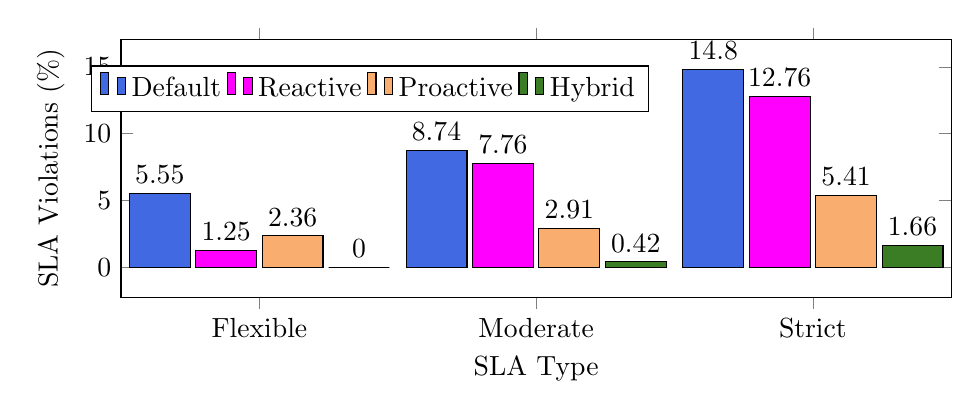
\begin{tikzpicture}
        \begin{axis}[
            height=0.4\linewidth,
            width=\linewidth,
            x tick label style={
                /pgf/number format/1000 sep=},
            ylabel=SLA Violations (\%),
            xlabel=SLA Type,
            enlarge x limits=0.25,
            enlarge y limits=0.15,
            legend style={at={(0.3,0.9)},
            anchor=north,legend columns=-1},
            ybar,
            bar width=22pt,
            symbolic x coords={Flexible, Moderate, Strict},
            xtick=data,
            nodes near coords,
            nodes near coords align={vertical},
        ]
        \addplot [fill = RoyalBlue]
        coordinates {(Flexible,5.55) (Moderate,8.74) (Strict,14.8)};
        \addplot [fill = Magenta]
        coordinates {(Flexible,1.25) (Moderate,7.76) (Strict,12.76)};
        \addplot [fill = Apricot]
        coordinates {(Flexible,2.36) (Moderate,2.91) (Strict,5.41)};
        \addplot [fill = OliveGreen]
        coordinates {(Flexible,0.00) (Moderate,0.42) (Strict,1.66)};
        \legend{Default, Reactive, Proactive, Hybrid}
        \end{axis}
    \end{tikzpicture}
\end{minipage}
\end{center}

Figure \ref{fig:exp1-sla-violation-bar} shows the SLA violations for the three different categories done on the GET API experiment. The flexible percentages were taken from the data taken from the five-day experiment using the 150 millisecond threshold, while the other two threshold values were extracted from the two-day experiments conducted for each. The default Kubernetes autoscaler performed the worst, with 5.55\% of all requests being above the SLA threshold. The proactive PPA algorithm came next with a violation rate of 2.36\%, with the number of violations being increased due to the complexity of the training model. The reactive THPA algorithm performed well, the low resource deployment, combined with the low overhead of GET requests ensured that it only violated the SLA thresholds of 1.25\% of requests. Finally, as seen above, the hybrid autoscaler performed the best out of the four algorithms, being able to serve all the requests with a 0\% SLA violation rate. This would qualify the hybrid architecture for a ``highly available'' SLA deployment.\par

While the flexible SLA threshold showed impressive results for three out of the four algorithms, the moderate threshold of 125 milliseconds was a more difficult constraint to maintain. The importance of mitigating or eliminating the cold start problem when it came to SLA latency was exposed in this threshold, as the default Kubernetes implementation and the reactive THPA autoscaler showed similarly poor results, violating 8.74\% and 7.76\% of requests respectively. On the contrary, the slower proactive PPA approach was able to demonstrate how mitigating the cold start problem while not being able to eliminate it completely could still have benefits, with the algorithm violating just 2.91\% of requests. Finally, the hybrid autoscaler still achieved the best results. There were violations at the beginning of the experiment, resulting in 0.42\% of requests being above the SLA threshold. However, this was quickly counteracted by the autoscaler controller, which modified the hyper-parameters to stabilize the latency. Once this was achieved, the hyper-parameters were dropped back down to the default values, and the auto-scaling continued as normal.\par

Finally, the strict SLA threshold of 100 milliseconds was tested, which proved extremely difficult to comply with. Once again, the default and reactive autoscalers performed significantly poorly, with 14.8\% and 12.76\% of requests not meeting the SLA threshold respectively. The proactive algorithm distinguished itself from the reactive ones, clearly showing the importance of the cold start problem, by only violating 5.41\% of the requests. However, in this scenario as well, the hybrid algorithm performed substantially better with only 1.66\% of violations. Even though the algorithm would occasionally violate the threshold, the combined approach, along with the controller's heuristic feedback was able to control the violation rate far better than the three baseline approaches. The total number of requests, along with the number of violations is provided in the table \ref{tab:exp1-sla-violation-count}.\par

%TC:ignore
\begin{table}
    \caption{SLA violation counts for \textit{home-timeline-service}}\label{tab:exp1-sla-violation-count}
    \centering
    \begin{tabular}{|l|l|l|l|}
        \hline
        Request Counts & Flexible & Moderate & Strict \\
        \hline
        Total  & \num[group-separator={,}]{2550000} & \num[group-separator={,}]{1220000} & \num[group-separator={,}]{1220000} \\
        \hline
        Default Violations & \num[group-separator={,}]{141525} & \num[group-separator={,}]{106628} & \num[group-separator={,}]{180560} \\
        Reactive Violations & \num[group-separator={,}]{31875} & \num[group-separator={,}]{94672} & \num[group-separator={,}]{155672} \\
        Proactive Violations & \num[group-separator={,}]{60180} & \num[group-separator={,}]{35502} & \num[group-separator={,}]{66002} \\
        Hybrid Violations & \num[group-separator={,}]{0} & \num[group-separator={,}]{5124} & \num[group-separator={,}]{20252} \\
         \hline
    \end{tabular}
\end{table}
%TC:endignore

\begin{comment}
\begin{figure}[htb]
    \centering
    \caption{SLA Violation Percentages For \textit{compose-post-service}}
    \label{fig:exp2-sla-violation-bar}
    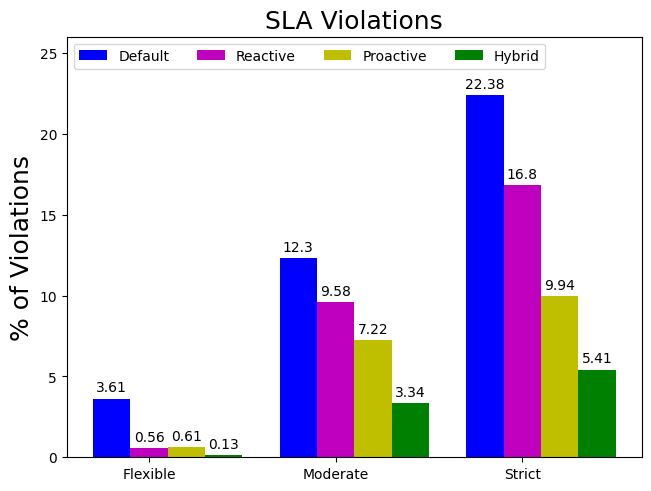
\includegraphics[width=0.6\linewidth]{Figures/Compose-Post-SLA-Violations.pdf}
\end{figure}


\begin{center}
\begin{minipage}{\linewidth}
    \captionof{figure}{SLA Violation Percentages For \textit{compose-post-service}}
    \label{fig:exp2-sla-violation-bar}
    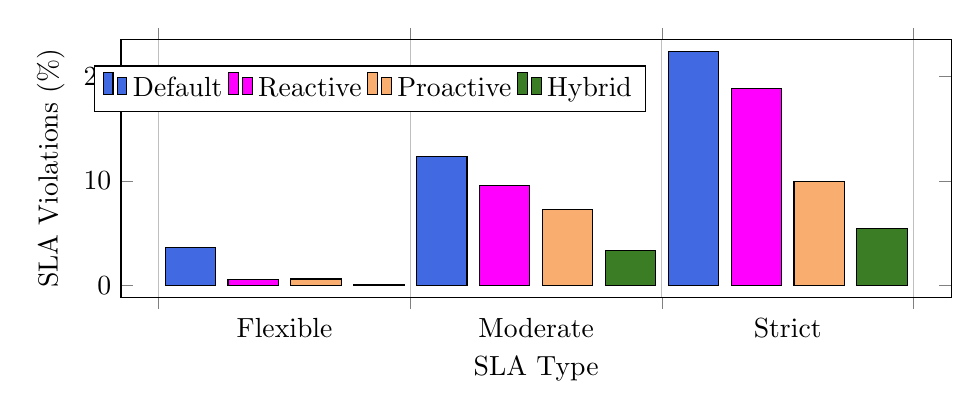
\begin{tikzpicture}
        \begin{axis}[
            height=0.4\linewidth,
            width=\linewidth,
            x tick label style={
                /pgf/number format/1000 sep=},
            ylabel=SLA Violations (\%),
            xlabel=SLA Type,
            enlargelimits=0.05,
            legend style={at={(0.3,0.9)},
            anchor=north,legend columns=-1},
            ybar interval=0.8,
            %symbolic x coords = {5,10,50,100,500,1000,DUMMY}
            xticklabels={Flexible, Moderate, Strict, DUMMY},
            xtick={5, 10, 15, 20},
        ]
        \addplot [fill = RoyalBlue]
        coordinates {(5,3.61) (10,12.3) (15,22.38) (20, 0)};
        \addplot [fill = Magenta]
        coordinates {(5,0.56) (10,9.58) (15,18.8) (20, 0)};
        \addplot [fill = Apricot]
        coordinates {(5,0.61) (10,7.22) (15,9.94) (20, 0)};
        \addplot [fill = OliveGreen]
        coordinates {(5,0.13) (10,3.34) (15,5.41) (20, 0)};
        \legend{Default, Reactive, Proactive, Hybrid}
        \end{axis}
    \end{tikzpicture}
\end{minipage}
\end{center}
\end{comment}

\begin{center}
\begin{minipage}{\linewidth}
    \captionof{figure}{SLA violation percentages for \textit{compose-post-service}}
    \label{fig:exp2-sla-violation-bar}
    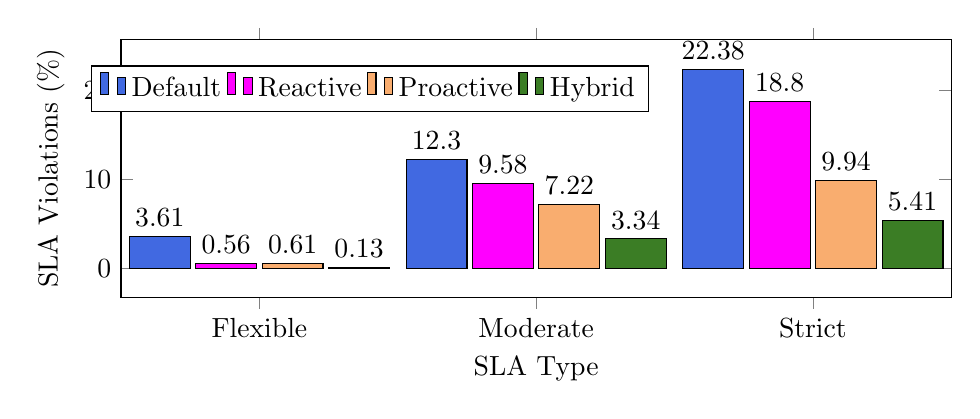
\begin{tikzpicture}
        \begin{axis}[
            height=0.4\linewidth,
            width=\linewidth,
            x tick label style={
                /pgf/number format/1000 sep=},
            ylabel=SLA Violations (\%),
            xlabel=SLA Type,
            enlarge x limits=0.25,
            enlarge y limits=0.15,
            legend style={at={(0.3,0.9)},
            anchor=north,legend columns=-1},
            ybar,
            bar width=22pt,
            symbolic x coords={Flexible, Moderate, Strict},
            xtick=data,
            nodes near coords,
            nodes near coords align={vertical},
        ]
        \addplot [fill = RoyalBlue]
        coordinates {(Flexible,3.61) (Moderate,12.3) (Strict,22.38)};
        \addplot [fill = Magenta]
        coordinates {(Flexible,0.56) (Moderate,9.58) (Strict,18.8)};
        \addplot [fill = Apricot]
        coordinates {(Flexible,0.61) (Moderate,7.22) (Strict,9.94)};
        \addplot [fill = OliveGreen]
        coordinates {(Flexible,0.13) (Moderate,3.34) (Strict,5.41)};
        \legend{Default, Reactive, Proactive, Hybrid}
        \end{axis}
    \end{tikzpicture}
\end{minipage}
\end{center}

Figure \ref{fig:exp2-sla-violation-bar} depicts the SLA violations for all four algorithms for the three SLA categories done on the POST API experiment. Once again, the flexible percentages were derived from the data taken during the five-day experiment using the 1000 millisecond threshold, while the moderate (900 milliseconds) and strict (800 milliseconds) violations were derived from the two-day workload above.\par

As seen above, for the flexible category, the default Kubernetes autoscaler performed the worst, with 3.61\% of the total requests resulting in an SLA violation. This also includes the requests which resulted in an error due to being dropped by the social network. The reactive and proactive algorithms performed comparatively similarly to each other, achieving a 0.56\% and 0.61\% violation rate respectively. The lenient threshold means that the proactive algorithm is unable to display its benefits when it comes to mitigating the cold start problem as compared to the reactive approach. Finally, the hybrid approach achieved a 0.13\% SLA violation rate. This results in approximately 99.9\% availability for the system, indicating that even for a difficult auto-scaling task such as for the POST request scenario, the hybrid algorithm is capable of achieving near ``high availability''.\par

The moderate SLA threshold proved far more difficult for all the algorithms to adhere to. Once again, the default Kubernetes autoscaler performed the worst of all four, failing to adhere to the SLA constraint for 12.3\% of the requests. Here, the proactive autoscaler was able to demonstrate the importance of mitigating the issue of cold start. It was able to achieve a 7.22\% of SLA violations, which was far lower than the 9.58\% seen for the reactive autoscaler. However, once again, the hybrid solution proved to be the most capable of auto-scaling in this scenario, achieving an SLA violation rate of just 3.34\%.

Finally, the extremely challenging strict threshold was tested. The default Kubernetes autoscaler was unable to cope with such a threshold, violating this threshold for over one-fourth of the requests, with a 22.38\% violation rate. Once again, the proactive algorithm outperformed the reactive one, achieving a 9.94\% violation rate as compared to the 18.8\% of the reactive algorithm. Finally, the hybrid algorithm performed significantly better than all three baselines yet again, with a violation rate of just 5.41\%.\par

This meant that over the two experiments and three SLA thresholds, the hybrid approach served a minimum of 94.5\% of all requests in an SLA-compliant manner in the worst-case scenario while serving 100\% of them in the best case. Through this thorough testing and experimentation, the algorithm displayed its robustness and adaptability while requiring little to no customization by the user to achieve excellent results. The total number of requests, along with the number of request violations for the second experiment is displayed in table \ref{tab:exp2-sla-violation-count}.\par

%TC:ignore
\begin{table}
    \caption{SLA violation counts for \textit{compose-post-service}}\label{tab:exp2-sla-violation-count}
    \centering
    \begin{tabular}{|l|l|l|l|}
        \hline
        Request Counts & Flexible & Moderate & Strict \\
        \hline
        Total  & \num[group-separator={,}]{2550000} & \num[group-separator={,}]{1220000} & \num[group-separator={,}]{1220000} \\
        \hline
        Default Violations & \num[group-separator={,}]{92055} & \num[group-separator={,}]{150060} & \num[group-separator={,}]{273036} \\
        Reactive Violations & \num[group-separator={,}]{14280} & \num[group-separator={,}]{116876} & \num[group-separator={,}]{229360} \\
        Proactive Violations & \num[group-separator={,}]{15555} & \num[group-separator={,}]{88084} & \num[group-separator={,}]{121268} \\
        Hybrid Violations & \num[group-separator={,}]{3315} & \num[group-separator={,}]{40748} & \num[group-separator={,}]{66002} \\
         \hline
    \end{tabular}
\end{table}
%TC:endignore

Thus for the two experiments, and on three different SLA thresholds, it can be comprehensively concluded that the hybrid approach proved to be the best autoscaler when it came to an edge deployment with minimal resources available. Furthermore, the algorithm was adaptable and able to display considerably improved performance in comparison with other reactive and proactive approaches. It was able to achieve this with minimal parameter configurations required by the user, and minimizing the cost of deploying and maintaining the edge architecture.
